%%%%%%%%%%%%%%%%%%%%%%%%%%%%%%%%%%%%%%%%%%%%%%%%%%%%%%%%%%%%%%%%%%%%%%%%%%%%%%%%
%					     	M.Sc. Thesis - (C)
%				      ALEXANDRU N. IOANA, 2020-2021
%%%%%%%%%%%%%%%%%%%%%%%%%%%%%%%%%%%%%%%%%%%%%%%%%%%%%%%%%%%%%%%%%%%%%%%%%%%%%%%%

% Print on A4 paper, base font size 12pt
\documentclass[a4paper,12pt]{report}

\usepackage[top=3.81cm,bottom=3cm,inner=3.5cm,outer=2.54cm]{geometry}

\setcounter{secnumdepth}{4}

% Actual font selection
\usepackage{pxfonts} % bookman | pxfonts | cmbright

% Include support for US english hyphenation (if installed on your system)
\usepackage[USenglish]{babel}

% Include support for correct printing of romanian characters
\usepackage[T1]{fontenc}
\usepackage{ucs}
\usepackage[utf8]{inputenc}

% Include support for graphics and code highlighting
\usepackage[pdftex]{color,graphicx}
\usepackage{minted}

% Include support for wrapping figures left or right
\usepackage{wrapfig}

% Use colors
\usepackage{xcolor}

% Include support for hyperlinks in the document
\PassOptionsToPackage{hyphens}{url}
\usepackage{hyperref}
\usepackage{url}
\hypersetup{unicode=true,%
	colorlinks=true,%
	citecolor=black,%
	filecolor=black,%
	linkcolor=black,%
	urlcolor=blue,%
	breaklinks=true}
	
% Include support for PDFs
\usepackage{pdfpages}

\setcounter{tocdepth}{3}

% Support special symbols
\usepackage{wasysym}
\usepackage{marvosym}
\usepackage{fontawesome}

% Support table formatting
\usepackage{tabularx}

% Allow left-justified/centered/right-justified table cells with fixed size
\usepackage{array}
\usepackage{ragged2e}
\newcolumntype{L}[1]{>{\RaggedRight\hspace{0pt}}p{#1}}
\newcolumntype{C}[1]{>{\Centering\hspace{0pt}}p{#1}}
\newcolumntype{R}[1]{>{\RaggedLeft\hspace{0pt}}p{#1}}

% Indent first paragraph
\usepackage{indentfirst}

% Describing algorithms
\usepackage[figure,longend,lined,boxed]{algorithm2e}

% Settings for using source highlighter
\usepackage{alltt}
\usepackage{marvosym}

\newcommand{\hlstd}[1]{\textcolor[rgb]{0,0,0}{#1}}
\newcommand{\hlnum}[1]{\textcolor[rgb]{0.53,0,0.13}{#1}}
\newcommand{\hlesc}[1]{\textcolor[rgb]{1,0,1}{\bf{#1}}}
\newcommand{\hlstr}[1]{\textcolor[rgb]{0.67,0.27,0}{#1}}
\newcommand{\hldstr}[1]{\textcolor[rgb]{0,0.53,0}{#1}}
\newcommand{\hlslc}[1]{\textcolor[rgb]{0.93,0.47,0}{#1}}
\newcommand{\hlcom}[1]{\textcolor[rgb]{1,0.53,0}{#1}}
\newcommand{\hldir}[1]{\textcolor[rgb]{0,0.53,0.27}{\bf{#1}}}
\newcommand{\hlsym}[1]{\textcolor[rgb]{0,0,0}{\bf{#1}}}
\newcommand{\hlline}[1]{\textcolor[rgb]{0.2,0.2,0.2}{#1}}
\newcommand{\hlkwa}[1]{\textcolor[rgb]{0.4,0.07,0.07}{\bf{#1}}}
\newcommand{\hlkwb}[1]{\textcolor[rgb]{0,0,0.4}{\bf{#1}}}
\newcommand{\hlkwc}[1]{\textcolor[rgb]{0,0,0.4}{#1}}
\newcommand{\hlkwd}[1]{\textcolor[rgb]{0,0.27,0.4}{#1}}
\definecolor{bgcolor}{rgb}{1,1,1}

% Setup some new commands for easier image inserting and figure referencing
% Creates the text for referring to the figure identified by the key given as
% the first argument.
\newcommand{\figname}[1]{\emph{figura \ref{#1}}}

% Inserts a new figure, with these parameters:
%	#1 - filename of the figure to be inserted
%	#2 - caption for the figure
%	#3 - label for the figure (used in \ref-ing the figure)
\newcommand{\insfig}[3]{
	\begin{figure}[!htb]
		\begin{center}
			\fbox{
				%\includegraphics[width=0.75\textwidth]{#1}
 				\includegraphics{#1}
			}
			\caption{#2\label{#3}}
			
	    \end{center}
	\end{figure}
}

% Inserts a new figure, with these parameters:
%	#1 - filename of the figure to be inserted
%	#2 - caption for the figure
%	#3 - label for the figure (used in \ref-ing the figure)
%	#4 - fraction of the text width occupied by the figure
\newcommand{\insfigw}[4]{
	\begin{figure}[!htb]
		\begin{center}
			%\fbox{
				\includegraphics[width=#4\textwidth]{#1}
			%}
			\caption{#2\label{#3}}
			
	    \end{center}
	\end{figure}
}

% Inserts a new figure, with these parameters:
%	#1 - filename of the figure to be inserted
%	#2 - caption for the figure
%	#3 - caption for display in the list of figures
%	#4 - label for the figure (used in \ref-ing the figure)
%	#5 - fraction of the text width occupied by the figure
\newcommand{\insfigshw}[5]{
	\begin{figure}[!htb]
		\begin{center}
			\fbox{
				\includegraphics[width=#5\textwidth]{#1}
			}
			\caption[#3]{#2\label{#4}}
			
	    \end{center}
	\end{figure}
}

% Abbreviations, Glossary & Appendix
\usepackage[acronym]{glossaries}
\makeglossaries
\newacronym{ui}{UI}{User Interface}

\newacronym{ux}{UX}{User Experience}

\newacronym{upb}{UPB}{University POLITEHNICA of Bucharest}

\newacronym{acs}{ACS}{Faculty of Automatic Control and Computer Science}

\newacronym{ta}{TA}{Teaching Assistant}

\newacronym{os}{OS}{Operating System}

\newacronym{api}{API}{Application Programming Interface}

\newacronym{ci}{CI}{Continuous Integration}

\newacronym{cd}{CD}{Continuous Deployment}
\newglossaryentry{moodle}
{
        name=Moodle,
        description={(Modular Object-Oriented Dynamic Learning Environment) is an open source, online courseware platform that runs under all major operating systems. Developed by Martin Dougiamas at Curtin University in Australia, Moodle provides all the necessary tools for educators to create a virtual classroom via the Internet \cite{crosslin2010course}}
}

\newglossaryentry{json}
{
        name=JSON,
        description={(JavaScript Object Notation) is a lightweight data-interchange format based on defining key-value pairs}
}

\newglossaryentry{firebase}
{
        name=Firebase,
        description={is a mobile and web application development platform developed by Firebase, Inc. in 2011, then acquired by Google in 2014}
}

\newglossaryentry{covid19}
{
        name=COVID-19,
        description={or coronavirus disease 2019 is a respiratory virus caused by the \textit{Severe acute respiratory syndrome coronavirus 2 (SARS-CoV-2)} strain of coronavirus}
}

\newglossaryentry{smis}
{
        name=SMIS,
        description=a web archive of EU-funded projects published by the Romanian Ministry of Public Finance
}
\usepackage{caption}
\usepackage[toc,page]{appendix}

% Setting headers
\usepackage{fancyhdr}
\pagestyle{fancy}
\fancyhead{}
\fancyhead[L]{\nouppercase{\leftmark}}
\fancyhead[RO]{\nouppercase{\rightmark}}
\setlength\headheight{14.5pt}

% Set spacing at 1.5lines
\linespread{1.3}

\usepackage{pdflscape}
\usepackage{graphicx,xcolor}
\usepackage{textgreek}

% This allows using acronyms and glossary entries in the chapter name
\pdfstringdefDisableCommands{
  \def\acrshort#1{<#1>}
  \def\acrlong#1{<1>}
  \def\gls#1{<1>}
}

% Allow using \paragraph as a sort of \subsubsubsection
\usepackage{titlesec}

\setcounter{secnumdepth}{4}

\titleformat{\paragraph}
{\normalfont\normalsize\bfseries}{\theparagraph}{1em}{}
\titlespacing*{\paragraph}
{0pt}{3.25ex plus 1ex minus .2ex}{1.5ex plus .2ex}

% Document begins here
\begin{document}

% Create title page
\thispagestyle{empty}
\begin{center}
\large
UNIVERSITY POLITEHNICA OF BUCHAREST \\
FACULTY OF AUTOMATIC CONTROL AND COMPUTERS \\
\vspace{\stretch{1}}

\begin{tabular}[t]{@{}l}
	
\includegraphics[scale=0.16]{figures/logos/upb.png}
\end{tabular}
\hfill
\begin{tabular}[t]{l@{}}
	
\includegraphics[scale=0.3]{figures/logos/cse.png}
\end{tabular}
\vfill\noindent

{\LARGE
	\textbf{Multi-source university news aggregator}
	\textbf{Agregator de știri universitare din mai multe surse}
}

\vspace{3cm}
\textbf{Graduate:}\\
Ștefan-Andrei Popa

\bigskip
\bigskip

\textbf{Thesis supervisors:}\\
Lecturer Dr. Alexandru Grădinaru \\
Engr. Ioana Alexandru \\

\vspace{\stretch{2}}
Bucharest \\
2022 \\
\vspace*{1cm}
\end{center}


% Insert the abstract
\vspace*{\fill}
\noindent

\textit{The university is a complex environment with many creative people having as a disadvantage the fact that it sometimes develops chaotically. This development is visible in the vast array of software applications meant to assist students. Over time in our university, many such platforms were developed, including the university website, the faculty website, websites of different student organizations, wikis created by professors or departments, and the official course platform. This variety turned into an information overload for students who are expected to be aware of everything that is posted on these websites, to discern between relevant information and spam, while also busy attending courses and completing assignments.}

\textit{We believe that students themselves can address this issue by using the power of the community to flag and organize important information from these websites, disseminate it to relevant colleagues and help each other get through the labyrinth of information existing in the university.}

\textit{With this goal in mind, this paper describes a collaborative app that allows students to better organize their time and schedule by collectively identifying the most useful information from the university's sources and intelligently sharing it with their peers.}

\vspace*{\fill}

% Insert the table of contents
\tableofcontents

% Include list of figures and tables
\clearpage
\addcontentsline{toc}{chapter}{List of figures}
\listoffigures
\newpage
\addcontentsline{toc}{chapter}{List of tables}
\listoftables
\newpage

\chapter{Introduction} \label{chapter1}

\section{Motivation} \label{1:motivation}

    According to Kevin Kelly \cite{kelly2010technology}, \textit{technology is an extension of life.} Its roots in our day to day lives go so deep that, for most of us, it is impossible or extremely difficult to even imagine life without technology. It has slithered its way into our jobs \cite{lewis1996studying}, our commute \cite{kairi2019technology}, even our nutrition \cite{lewis2010role} and personal lives \cite{mcquillen2003influence}. It should come as no surprise that it has become a huge part of students' lives, which is what we will be focusing on hereafter.
    
    ~
    
    Due to the rapid pace in which new and better technologies replace the old ones, as well as the existence of a variety of tools that serve more or less the same purpose, students nowadays find themselves flooded with a plethora of platforms and resources provided by their faculty.
    
    The emergence of new and better tools that replace old ones often implies that some people will continue to use the old tools (or even "analogue" tools instead of "digital" ones) out of habit, while other, more progressive people will immediately switch to the new ones. This leads to a discrepancy in the platforms used by professors for the same purpose, which in turn overwhelms students to the point where some even drop out.
    % TODO: Link to case study with used technlogies in ACS
    
    In order to cope with the huge influx of information (new knowledge, as well as administrative details), students oftentimes turn to each other for help and assistance. This process is informal in nature, taking place either face to face or through social media platforms.
    % TODO: Link to case study with socialization in ACS
    \clearpage
    This paper proposes a cross-platform mobile application which aims to act as a compendium for the various resources offered by the university for the students, as well as provide an easy-to-use, intuitive platform for collaboration.

\section{Environment} \label{1:environment}

    For the purpose of this paper and the application prototype, we will be analyzing the case of one of the 15 faculties\footnote{https://upb.ro/en/faculties/} of \textbf{\acrlong{upb}} in Romania, namely the \textbf{\acrlong{acs}}. From here on out, we will be referring to the larger engineering institution as \textit{the university} or \textit{\acrshort{upb}}, and to the computer science faculty as \textit{the faculty} or \textit{\acrshort{acs}}.
    
    \subsection{Student/user profile} \label{2:student_profile}
    
        The student using this app has the following characteristics:
        \begin{itemize}
            \item an ongoing \textbf{Bachelor's/Master's degree} in computer science
            \item average to high \textbf{digital proficiency}, common for computer science students%, therefore usage instructions should be minimal.
            \item proficiency in either \textbf{Romanian or English}, the two languages that the institution provides courses in%, therefore the application
            \item an age between \textbf{18 and 25 years}
        \end{itemize}
        
    \subsection{Student body structure} \label{1:student_body_structure}
    
        The faculty provides Bachelor's, Master's and Doctoral science degrees. We are interested in the B.Sc. and M.Sc. degrees, each of which are split into a couple of \textit{domains}. They last for four and two years respectively.
        
        For the \textbf{B.Sc.}, each domain has its own separate curriculum, and the students are organised hierarchically into \textit{series}, which are comprised of up to 5 \textit{groups}, which in turn can be split into two \textit{subgroups} each.
        
        For the \textbf{M.Sc.}, each domain hosts a number of master's programs, and each program corresponds to a single \textit{series} of students which is not split further.
        
        Each \textit{series} and each \textit{group} have a student representative who acts as a link between the corresponding group of students and the faculty, and is tasked with things like passing on important information, keeping in touch with the Student Office staff and making sure the contracts are signed by all students each semester.
    
    \subsection{University platforms} \label{1:university_platforms}
    
        The main platforms that the University staff use to provide resources to the students are:
        
        \begin{itemize}
            \item \textbf{the official university website} for general university information such as the campus map and academic calendar
            \item \textbf{the official faculty website} for the curriculum, certain announcements and timetable information
            \item \textbf{various course/wiki websites} for class resources
            \item \textbf{a \gls{moodle} instance} for class-related announcements, discussions and assignments
            \item \textbf{the university's administrative website} for the student contract, personal information and grades
            \item \textbf{several automated-testing environments} for coding assignments
        \end{itemize}
    
        Most of the aforementioned platforms can be accessed using a single set of credentials provided by the University upon admission.
        
    \subsection{Class structure} \label{1:class_structure}
    
    A student's schedule is comprised of three main types of classes:
    
    \begin{itemize}
        \item \textbf{lectures}: theoretical classes taught by professors or lecturers, which take part in a lecture hall and in which a whole series (or two, in some cases) of students participates
        \item \textbf{laboratories}: practical classes taught by professors, lecturers (rarely) or \acrshort{ta}s (\acrlong{ta}s), which require a computer or other external tools (e.g. lab equipment, electrical equipment etc.), which take part in dedicated lab rooms and in which only a group or subgroup of students participates
        \item \textbf{seminars}: practical classes taught by professors or lecturers, which only require pen, paper and a whiteboard, which take part in classrooms and in which only a group or subgroup of students participates
    \end{itemize}
    
    The main forms of evaluation are: theoretical exams, homeworks, projects, tests, practical exams and research assignments.
        
\section{Proposed functionalities} \label{1:functionalities}

    Given the environment described in section \ref{1:environment}, we can propose a number of main functionalities for the application:
    
    \begin{itemize}
        \item \textbf{authentication} (ideally linked to the common credentials used for the other platforms)
        \item \textbf{localization}: the application should provide a \acrshort{ui} (\acrlong{ui}) in both Romanian (for local students) and English (for international students)
        \item the possibility to \textbf{access, modify and filter a list of platforms provided by the university} (see section \ref{1:university_platforms}), as well as view information about their use
        \item the possibility to collaboratively \textbf{create and edit a timetable} which includes class information as well as various events
        \item \textbf{campus map and navigation information}
        \item \textbf{news, FAQs and other relevant information} that students can contribute to
    \end{itemize}

\section{Goals} \label{1:goals}

    The application aims to make students' lives easier by providing a single point of access for all university resources and needs, supported by the students, for the students. It should be intuitive and easy to use, as well as allow customization for any kind of student.
    
    Above all, the application should be particularly helpful for freshman students by offering an easy way to find out anything they want to know about the ins and outs of their new university life.
    
    Ultimately, the application aims to become an integral part of students' lives and contribute to their education, all the while decreasing the feelings of anxiety caused by being bombarded with new, often disorganised information.

\section{Outline} \label{1:outline}
    TODO
\chapter{State of the Art} \label{chapter2}

Currently, in the industry, there exists a large number of applications aiming to help students of all ages organise their school lives better. These range from \textit{apps made specifically for a certain university} to \textit{generic, highly customizable applications} meant to tackle a student's needs regardless of the institution they study at. In addition to these, there exist a number of \textit{productivity tools that are not targeted specifically at students}, but which are frequently used by them for school-related activities. A 2013 study\cite{chen2013exploring} shows that students generally use a large variety of different mobile resources to help with their academic life.

We will attempt to analyze the pros and cons of each category mentioned above and pick the features that would be most appropriate for our application, in order to reach the goals described in section \ref{1:goals}.

Additionally, we will also be looking into the existing applications targeted for students at \acrshort{acs}/\acrshort{upb}, in order to plan a potential integration and collaboration and avoid re-inventing the wheel.

\section{University-specific applications} \label{2:uni_apps}

    \subsection{Overview} \label{2:uni_apps_overview}

        Many top universities from around the world nowadays leverage the popularity of mobile devices by offering their students an application (or a set of applications) for their university needs, as pictured in figure \ref{2:fig:uni_apps}. These often become indispensable, because a lot of the communication with the university is done solely through the application. They are usually meant to complement the university's official website as a mobile-friendly, feature-rich platform, and are generally available on both iOS and Android devices so that any student can have access to them.
        
        The most frequent features found within these applications are: university information and news (including syllabus, admissions and student accommodation information), class timetables and academic calendars, campus maps including canteen, library and shuttle information for universities that provide such amenities.
        
        \begin{figure}[ht]
            \centering
                 
\includegraphics[width=0.13\textwidth]{figures/uni_apps/store_entries/columbia.png}
                 
\includegraphics[width=0.13\textwidth]{figures/uni_apps/store_entries/mit.png}
                 
\includegraphics[width=0.13\textwidth]{figures/uni_apps/store_entries/notre_dame.png}
                 
\includegraphics[width=0.13\textwidth]{figures/uni_apps/store_entries/princeton.png}
                 
\includegraphics[width=0.13\textwidth]{figures/uni_apps/store_entries/stanford.png}
            \caption{University-specific applications on Google Play}
            \label{2:fig:uni_apps}
        \end{figure}
    
    \subsection{Case Study} \label{2:uni_apps_case_study}

        \begin{wrapfigure}{l}{0.23\columnwidth}
            \centering
            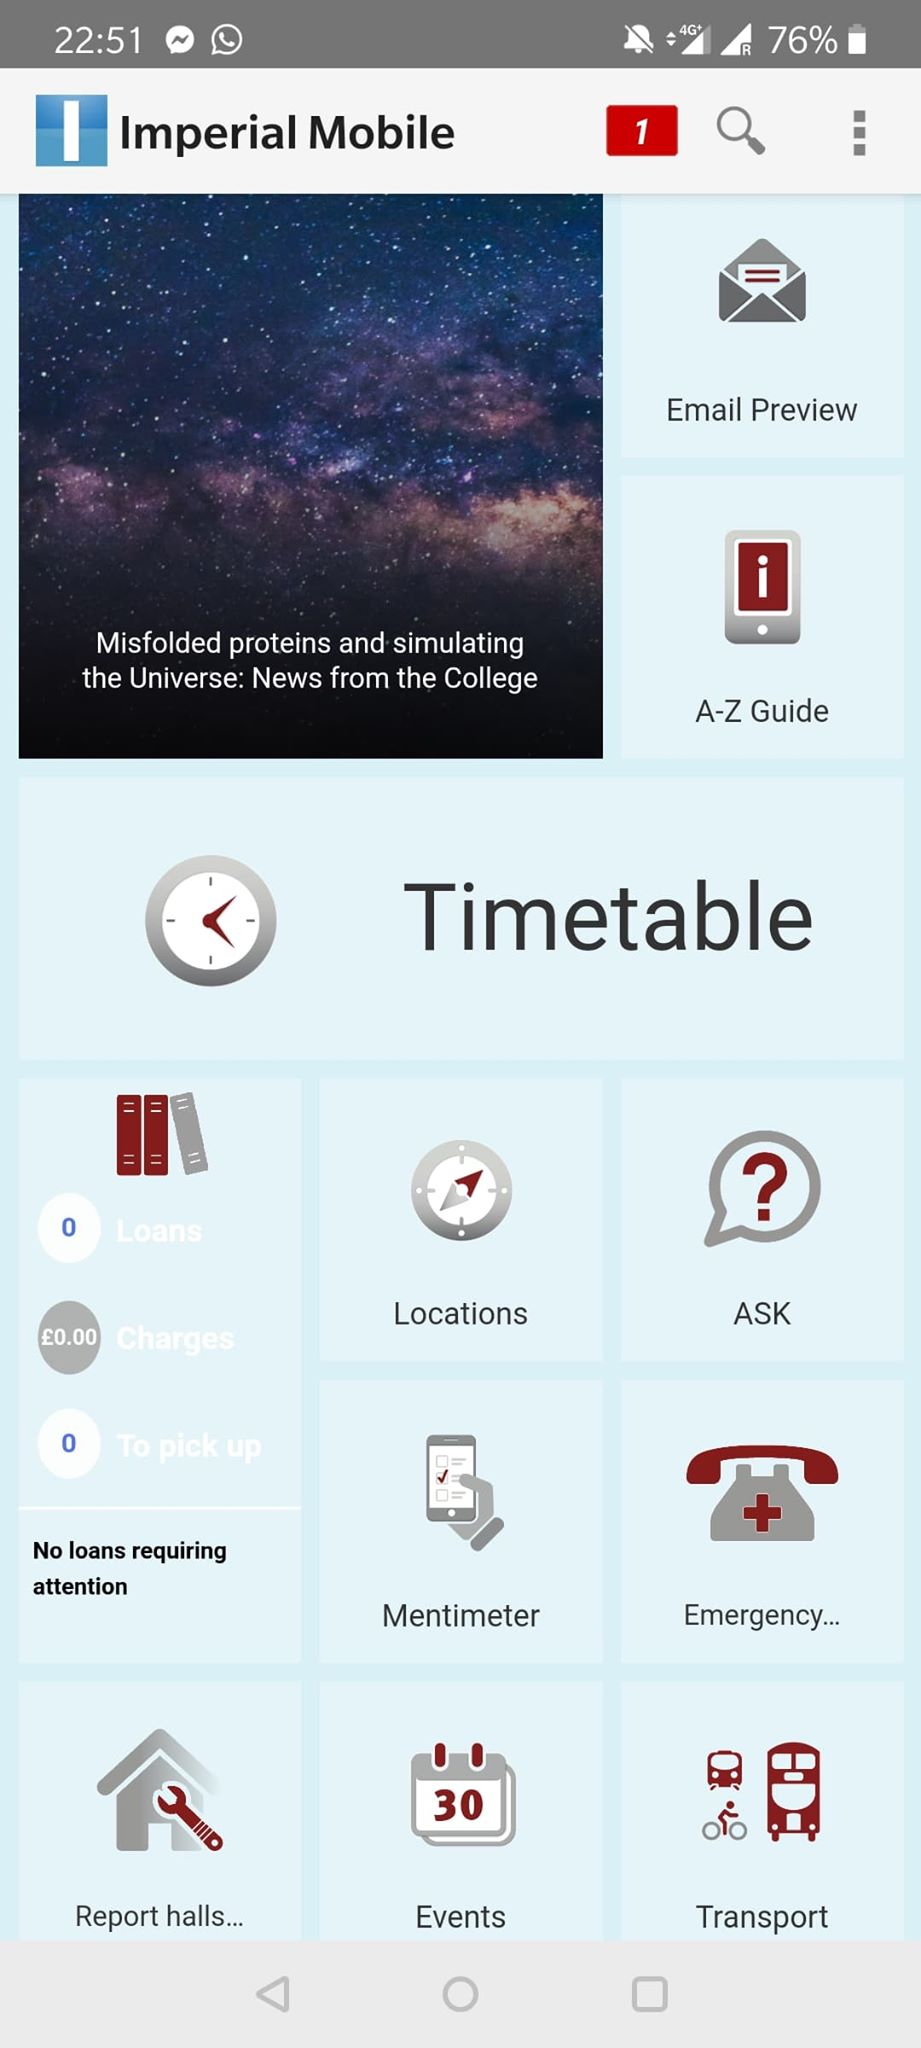
\includegraphics[width=0.23\columnwidth]{figures/uni_apps/screenshots/imperial.jpg}
            \captionsetup{labelsep=space, textformat=empty}
            \caption{Screenshot of the main page of the Imperial app}
            \label{2:fig:imperial_screenshot}
        \end{wrapfigure}
    
        We interviewed a third year Romanian medical engineering student at Imperial College London\footnote{https://www.imperial.ac.uk/} in order to learn more about their experience with the official university app (fig. \ref{2:fig:imperial_screenshot}). They admitted that the app played an important role in their adaptive process in the first year of university, because it provided important information about student halls of residence as well as incoming freshman events. They also pointed out that the main use of the app for them and their peers is to find out the timetable, but that they were bothered by the fact that it was a static table rather than a customizable one. Additionally, they mentioned that they wished they could import the events to any calendar application of choice (e.g. \textit{Google Calendar}\footnote{https://calendar.google.com/}, \textit{Microsoft Outlook}\footnote{https://outlook.office.com/}).
        
        \clearpage
        
        \begin{wrapfigure}{r}{0.25\columnwidth}
            \centering
            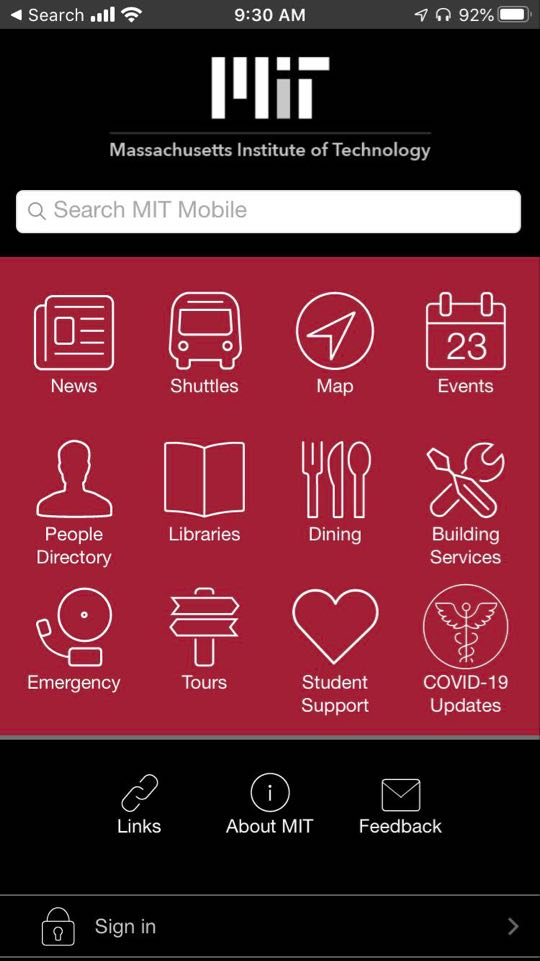
\includegraphics[width=0.25\columnwidth]{figures/uni_apps/screenshots/mit.jpg}
            \captionsetup{labelsep=space, textformat=empty}
            \caption{Screenshot of the main page of the MIT app}
            \label{2:fig:mit_screenshot}
        \end{wrapfigure}
        
        A graduate US computer science student at the Massachusetts Institute of Technology\footnote{https://www.mit.edu/} that we interviewed shared that the most used features of their university's app (fig. \ref{2:fig:mit_screenshot}) are the map, shuttle schedule, and dining menus. They also pointed out that the app is mostly useful (and therefore used by) freshman students, and that usage for older students is limited to the first day of classes if they have a class in a new building, or more regularly to check menus in dining halls, if they were on a meal plan. Furthermore, the student mentioned that the biggest problems they had with the university app were performance issues and outdated or inaccurate information (i.e. shuttle showing as running when it is not, or marked in a wrong location).
        
        An interviewed German computer science student at the Digital Engineering Faculty within the University of Potsdam\footnote{https://www.uni-potsdam.de/en/digital-engineering/} described a different experience. The faculty app is currently under development by a group of students including themselves. The application provides information about courses, faculty news as well as food options in the university's canteen and café, the last of which the student believes to be the most useful.
        
    \subsection{Pricing} \label{2:uni_apps_pricing}
    
        It is worth noting that, while some universities rely on teams of students and professors to develop their app, others prefer to hire professional teams offering development solutions. The costs of developing such an app vary, since there are countless companies offering specific services for universities - for example, as of May 2020, \textit{Guidebook}\footnote{https://guidebook.com/gb/pricing/} prices start at \$3,200, while \textit{buildfire}\footnote{https://buildfire.com/pricing/white-glove-pricing/} offers different plans that range from \$2,500 up to \$7,500 depending on requirements. Many companies opt against listing their prices publicly in favor of setting an appropriate price based on the specific client's needs (e.g. MODO\footnote{https://www.modolabs.com/products/modo-campus/}, Lets Nurture\footnote{https://www.letsnurture.com/services/mobile-app-development.html}).

\section{Generic education applications} \label{2:generic_apps}
    The market also offers a number of highly customizable class management solutions for students of all ages, such as \textit{School Assistant}\footnote{https://www.school-assistant.com/}, \textit{myHomework}\footnote{http://myhomeworkapp.com/} and \textit{ClassUp}\footnote{https://classup.plokia.com/} (all of which have over one million downloads on the Google Play Store\footnote{https://play.google.com/} alone).
    
    \subsection{Platforms} \label{2:generic_apps_platforms}
        The availability of these applications ranges from single-platform or single-\acrshort{os} (\textit{School Assistant} - Android devices only) to multi-platform or multi-\acrshort{os} (\textit{ClassUp} - Android and iOS devices) and all the way up to fully cross-platform (\textit{myHomework} has support for Android, iOS, Windows, MacOS, ChromeOS and FireOS, as well as a web version that can be accessed by any web-enabled device).
        
    \subsection{Features} \label{2:generic_apps_features}
        Most of these applications have a similar set of features, out of which the most notable are:
        
        \begin{itemize}
            \item customizable timetable that can be synced with other calendar applications, with the ability to define holidays and types of classes (fig. \ref{2:fig:school_assistant_timetable})
            \item assignment/homework/evaluation trackers with custom reminders
            \item tracker for class information such as professors who teach it, grades, associated events and notes (fig. \ref{2:fig:school_assistant_class})
        \end{itemize}
        
        Other features include automatically muting the phone during classes, importing/exporting data and customizing the looks of the application.
        
        All of this information needs to be manually inputted/modified by the user at the beginning of each semester and throughout the year as new events arise or changes are made.
        
        \clearpage
        
        \begin{figure}[!h]
            \centering
                \begin{minipage}[b]{0.39\textwidth}
                    \captionsetup{justification=centering}
                    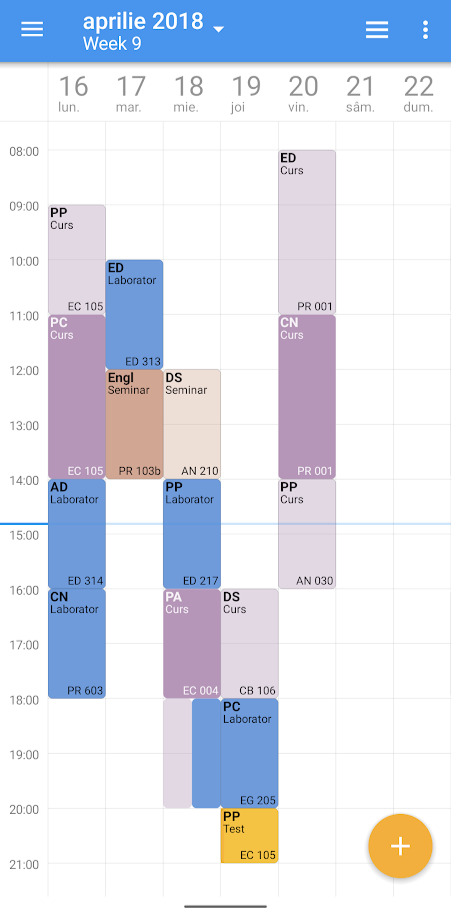
\includegraphics[width=\textwidth]{figures/uni_apps/features/school_assistant_timetable.png}
                    \caption{School Assistant: timetable page}
                    \label{2:fig:school_assistant_timetable}
                \end{minipage}
                \hfill
                \begin{minipage}[b]{0.39\textwidth}
                    \captionsetup{justification=centering}
                    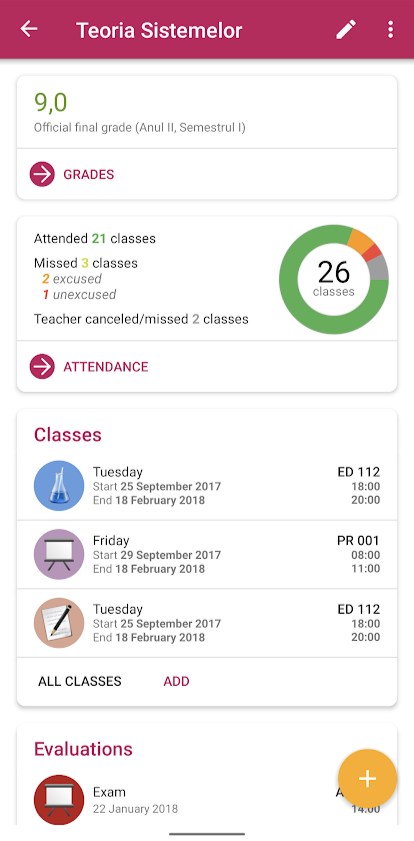
\includegraphics[width=\textwidth]{figures/uni_apps/features/school_assistant_class.png}
                    \caption{School Assistant: class details page}
                    \label{2:fig:school_assistant_class}
                \end{minipage}
                
        \end{figure}  
    
    \subsection{Pricing} \label{2:generic_apps_pricing}
        Unlike university-specific apps described in section \ref{2:uni_apps}, where costs are supported entirely by the university and usage is free for the students, generic applications usually require each student to pay for themselves. As is the trend with a lot of mobile applications nowadays, most of them are free initially (and might contain ads) and either offer a trial period or a limited number of features until the user upgrades to a paid version. \textit{School Assistant}, for instance, has another version of the app with more features, \textit{School Assistant +}, with an upfront cost of \$2.75. \textit{myHomework} has a subscription-based model: it provides a free version with limited functionality and advertisements, as well as the ability to upgrade to a \textit{Premium} version for \$4.99 a year. \textit{ClassUp}, on the other hand, is completely free and has no ads.
        
    \subsection{Caveats} \label{2:generic_apps_caveats}
        The biggest issue with all of these apps, stemming from their customizability, is that \textit{they need to be set up in order to work}. Unlike university-specific apps described in section \ref{2:uni_apps}, which generally "just work" as soon as you log in using your university credentials, for generic applications to be useful, the students need to manually input all of their classes, assignments, professor information and so forth. 
        
        Depending on the app, as well as the amount and complexity of the information that is to be inputted, this process can initially take from a few minutes to a few hours, and requires active updating by the student throughout the academic year (as new assignments are issued, classes change etc.). For most students, this is often more effort than it is worth, as we could observe from our \textbf{\nameref{chapter3}}, where out of over 200 students, only 3 said they were using a class management app (specifically, the 3 applications we chose as examples in this section).
        
        % TODO - Negative Google Play/App Store comments (word cloud?) 
        % https://helpcenter.octoparse.com/hc/en-us/articles/360027611891-Scrape-reviews-from-Google-Play

\section{Other productivity applications} \label{2:other_apps}
    % Doodle, Google Calendar, Teams, Outlook
    In order to stay on track, well-organised students often use productivity applications that aren't necessarily targeted for university specifically, but which get the job done. Our \textbf{\nameref{chapter3}} points out that out of over 200 students, about 60 regularly use Google Calendar or another calendar app to track their university tasks. 14 students mention using other productivity apps such as Trello\footnote{https://trello.com/} and other note-taking or todo-list applications (e.g. Google Keep\footnote{https://keep.google.com/}, ColorNote\footnote{https://www.colornote.com/}).
    
    The main reason why only 30\% of students opt for using a productivity app is that these have the same main disadvantage as generic university apps (described in section \ref{2:generic_apps_caveats}), namely they require active management and involvement. To keep track of their tasks, the other 70\% of students rely solely on their memory, reminders from colleagues and the limited resources provided by the university, such as the timetable (a simple spreadsheet) and the assignments listed in the \gls{moodle} calendar (which is only used for specific classes).

\section{Existing applications for our university} \label{2:existing_apps}
    Our goal being to "fill in the blanks" and provide students with tools that they would need to make their lives easier and that they don't already have, we looked into the existing applications (or existing attempts) for students in our target group.
    
    In the past few years, we have seen an increasing interest in providing a mobile application for students, with more and more students implementing small applications aiming to help their peers in various ways, and presenting them as projects for various classes, conferences (notably, the \acrshort{upb} Students Scientific Communications Session\footnote{https://upb.ro/sesiunea-de-comunicari-stiintifice-studentesti-2020-online/}) and even their Bachelor thesis (fig. \ref{2:fig:papers_aimed_at_students}). However, most of these projects do not go past the stage of a proof of concept due to lack of time from the initiating students and lack of support from the University (see subsection \ref{2:existing_apps_history}). In order to find out more, we interviewed some of these students and will be describing their work in subsections \ref{2:existing_apps_navigation} - \ref{2:existing_apps_other}.
    
    \begin{figure}[ht]
        \centering
             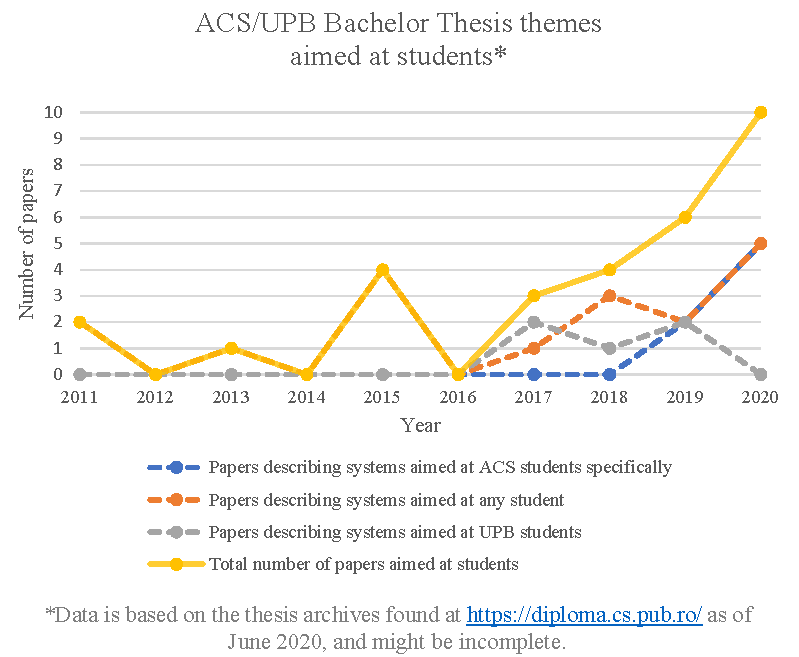
\includegraphics[width=0.8\textwidth]{figures/charts/papers_aimed_at_students.pdf}
        \caption{\acrshort{acs}/\acrshort{upb} Bachelor Thesis themes aimed at students}
        \label{2:fig:papers_aimed_at_students}
    \end{figure}
    
    \subsection{History} \label{2:existing_apps_history}
    As far as \acrshort{upb} and \acrshort{acs} are concerned, new platforms have a history of either not being officially accepted, or going through an extremely long process in order to eventually be adopted.
    
    \subsubsection{Current platforms} \label{2:existing_apps_history_current}
    The university's current platform for students to manage and view their enrollment information (including contracts, grades and accommodation),  \textit{studenti.pub.ro}, started back in 2007 as a small platform developed by students for managing housing requests for the university's student halls of residence. More much-needed functionality was added as time passed, and it slowly became an integral part of any \acrshort{upb} student's life. However, it hasn't seen a major update in a long time, with features such as requesting a proof of enrollment, graduation or other documents being greyed out and marked as \textit{coming soon} for the past few years.
    
    The university's \gls{moodle} platform was introduced through an EU-funded project called "E-learning and e-content curriculum platform for technical higher education" (project number 154/323, \gls{smis} code 4428), initiated for the whole university by an \acrshort{acs} professor in 2009. According to the project's official website\cite{upb2009elearning}, the percentage of university courses providing digital (e-learning) materials grew from 9\% (170 courses) up to 35\% (600 courses) thanks to the project.
    % TODO vmchecker? is it relevant?
    
    \subsubsection{\gls{covid19} response} \label{2:existing_apps_history_covid}
    Due to the 2020 pandemic with the new coronavirus (SARS-CoV-2), classes and evaluations in \acrshort{upb} were completely moved online starting in March, which lead to a sudden increase in usage for the university and the faculty's online platforms. Professors are now required to post all materials and assignments on \gls{moodle}, as opposed to before the pandemic when they had the ability to choose. With students having no other choice but to use the platform and attend online classes on Microsoft Teams\footnote{https://teams.microsoft.com/}, the number of users per hour soared. This initially led to issues due to the platform servers not being able to process such a large number of requests.
    
    % TODO data?
    Furthermore, some long-awaited changes came into effect thanks to the pandemic. For instance, requesting a document such as a proof of enrollment, an activity that previously required personally dropping off a hand-written request during the Student Office hours (9-11am), could finally be done virtually by simply sending an e-mail, as a result of the university building being closed for students due to the pandemic.
    
    Ultimately, we believe that this experience led to an important step in improving digitalization within the faculty and university, and we hope that future adoption processes will run more smoothly.
    
    \subsection{Navigation tools} \label{2:existing_apps_navigation}
    Since \acrshort{upb} prides itself with the largest campus in Romania\footnote{http://international.upb.ro/studenti-internationali/}, navigating the tens of buildings can be difficult for new students. While the map\footnote{http://international.upb.ro/campus/transport-eng/} helps, students often find themselves in need of a more interactive navigation solution. It should come as no surprise that computer science students would try to handcraft such a solution.
    
    \begin{figure}[!h]
        \centering
        \begin{minipage}[b]{0.49\textwidth}
            \captionsetup{justification=centering}
             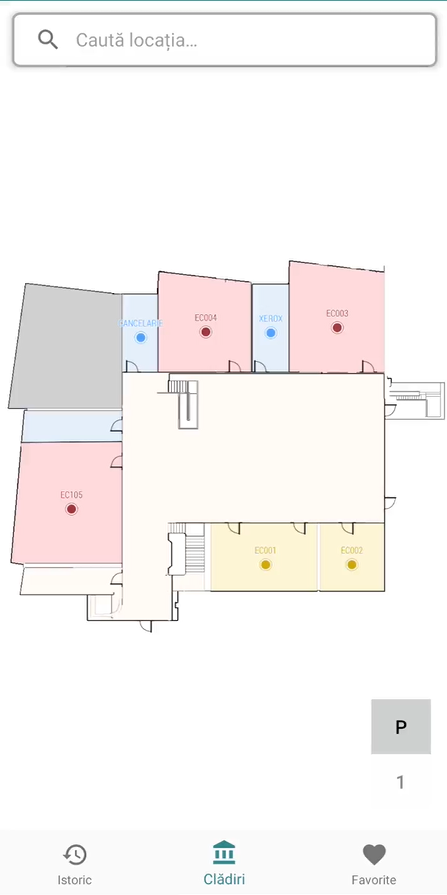
\includegraphics[width=0.49\textwidth]{figures/upb_apps/navigation/upb_campus_unpublished1.png}
             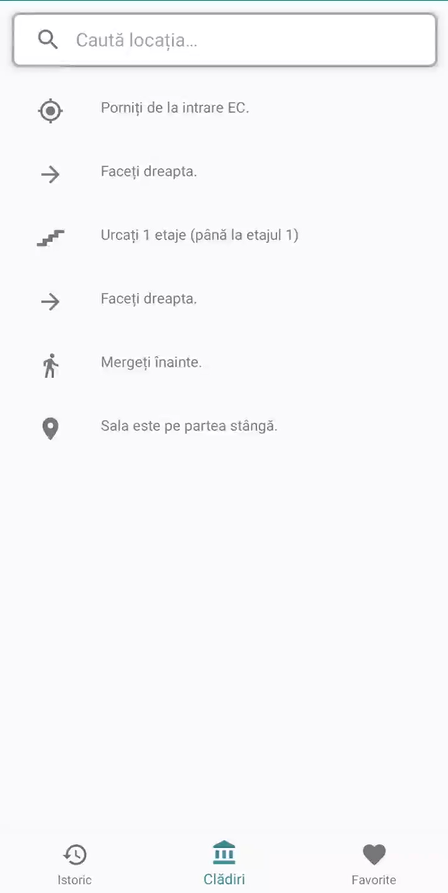
\includegraphics[width=0.49\textwidth]{figures/upb_apps/navigation/upb_campus_unpublished2.png}
            \caption{Unpublished \acrshort{upb} campus map application}
            \label{2:fig:upb_campus_unpublished}
        \end{minipage}
        \hfill
        \begin{minipage}[b]{0.49\textwidth}
            \captionsetup{justification=centering}
             
\includegraphics[width=0.49\textwidth]{figures/upb_apps/navigation/upb_campus_published1.png}
             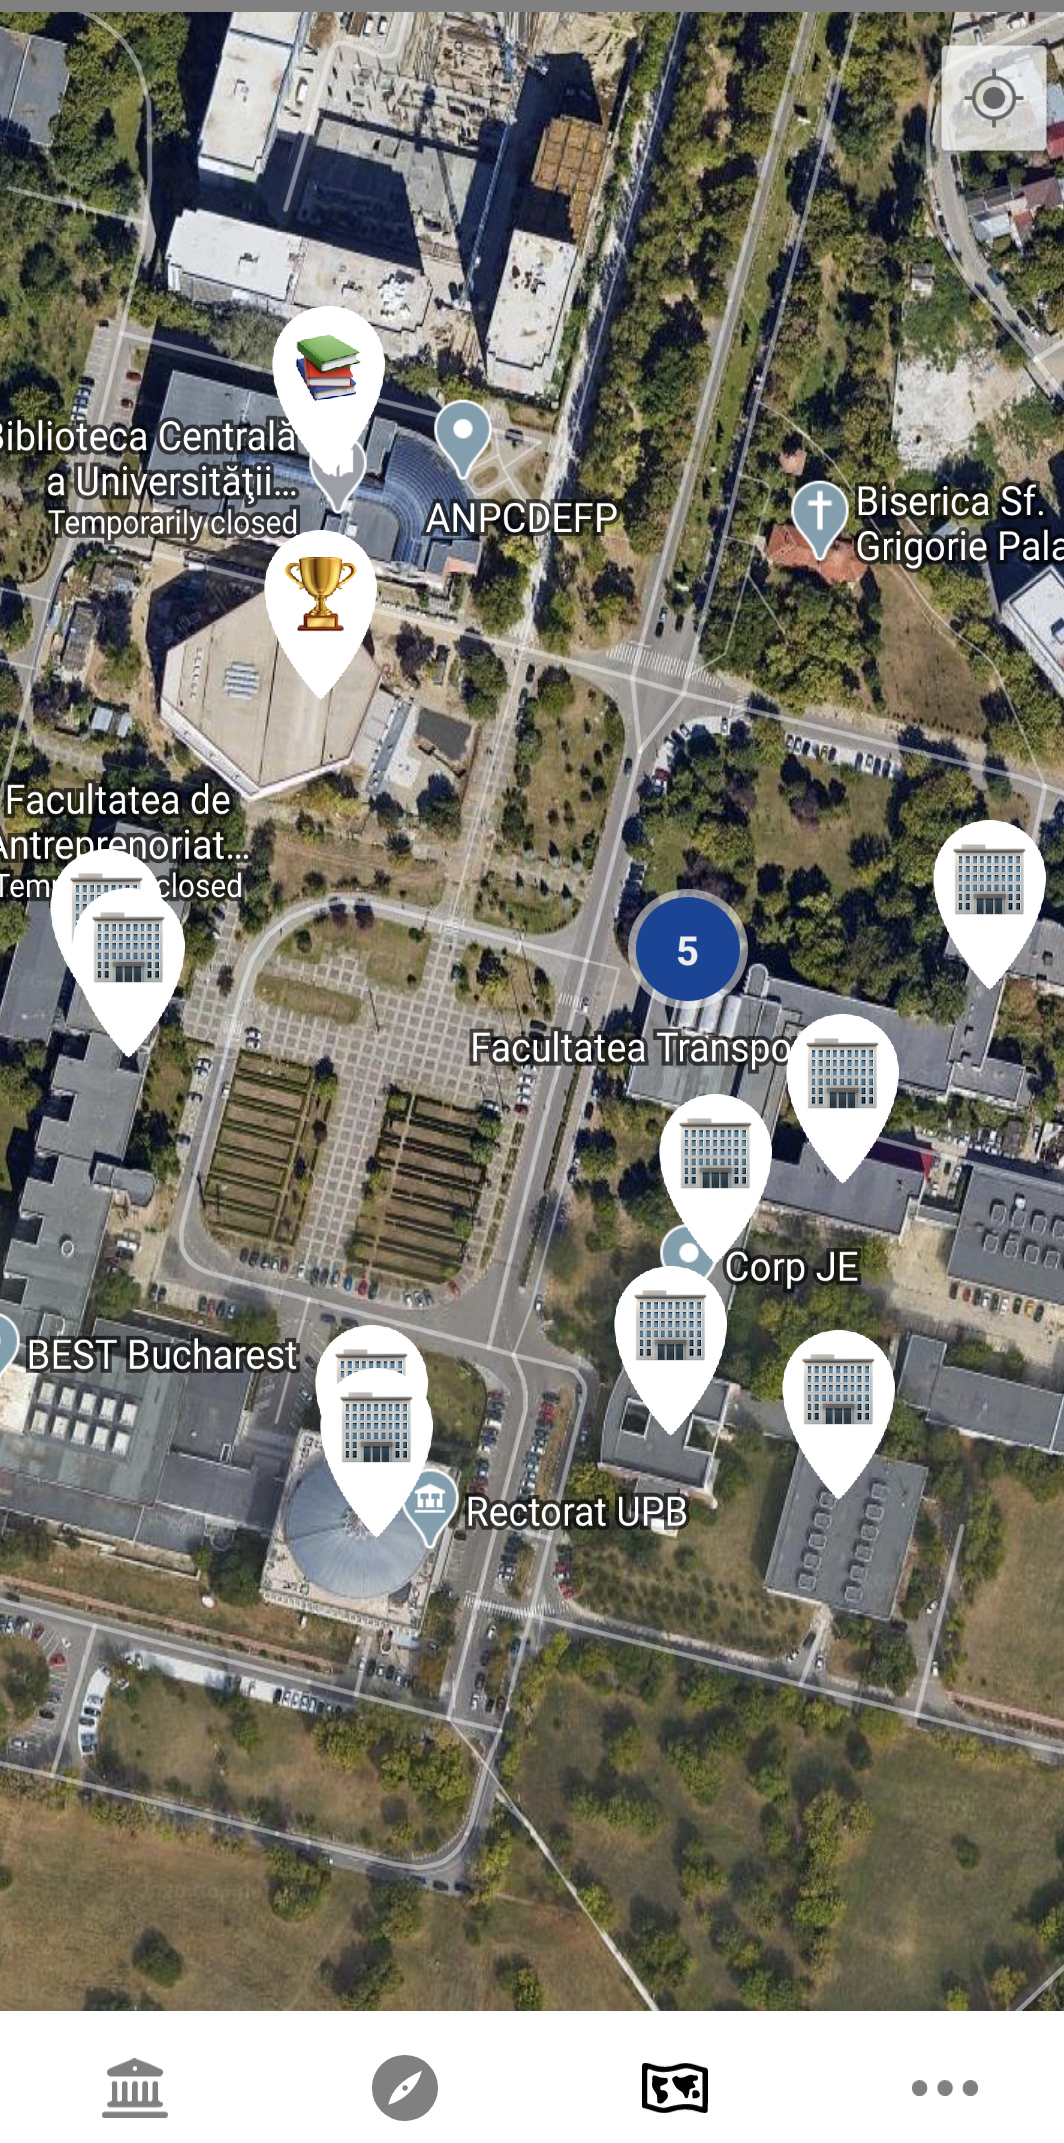
\includegraphics[width=0.49\textwidth]{figures/upb_apps/navigation/upb_campus_published2.png}
            \caption{Published \acrshort{upb} campus map application}
            \label{2:fig:upb_campus_published}
        \end{minipage}
    \end{figure}
    
    \clearpage
    
    In April 2019, a group of students attempted to create an Android app that provides indoors navigation instructions\footnote{https://github.com/IrinaM09/UPB}, as a group project for their software engineering class. The project, however, remained in the state of a simple proof of concept (fig. \ref{2:fig:upb_campus_unpublished}), due to the fact that there not being existing digital data of the room layout in the campus buildings meant that they had to manually write the information in the form of a graph in a \gls{json}\footnote{https://github.com/IrinaM09/UPB/blob/master/app/src/main/res/raw/nodes.json} file, a process which proved to be extremely tedious.
    
    Roughly a year later and completely separately, a student from the Faculty of Engineering in Foreign Languages\footnote{http://ing.pub.ro/en/} within \acrshort{upb}, with a passion for programming,  wrote a paper for the \acrshort{upb} Students Scientific Communications Session, won a prize and consequently published a campus map mobile application for both iOS and Android devices (fig. \ref{2:fig:upb_campus_published}), using the Apple Maps\footnote{https://developer.apple.com/maps/} and the Google Maps\footnote{https://developers.google.com/maps/documentation} APIs respectively.
    % TODO add paper info
    
    \subsection{Timetable/event tools} \label{2:existing_apps_timetable}
    Throughout the years, students have attempted to automatically extract class information from the university-provided timetable, in order to more easily add the events to their calendar application of choice. One such attempt was done by a Master's student in January 2019 as a project for a mobile computing class\footnote{https://github.com/laurentiustamate94/timetable-app}. However, the main difficulty they all encountered was that the timetable files are manually-written spreadsheets that don't have a set format each year, therefore there is no way to fully automate the extraction of events from these files, unless the professor that is in charge with designing the timetables agrees to standardize the whole process.
    
    In September 2019, a student who was tired of having to rely on colleagues or spend a large amount of time browsing \textit{Facebook} in order to find out what relevant events are taking place in or related to the university published an application called \textit{Politehnik}\footnote{https://politehnik.ro/}. This app promised to offer an easy way for students to keep track of what events are happening, as well as get notified about upcoming events they may be interested in. In spite of the fact that the app was solely promoted through faculty WhatsApp groups and that the features offered are only useful for a handful of students, the application saw a lot of interest from students (usage statistics pictured in fig. \ref{2:fig:politehnik_usage}, with the first steep rise being caused by the initial peer to peer promotion and subsequent spikes by in-app notifications). The events in the app are added manually by the developer, with users being able to suggest events through the app.
    
    \begin{figure}[ht]
        \centering
             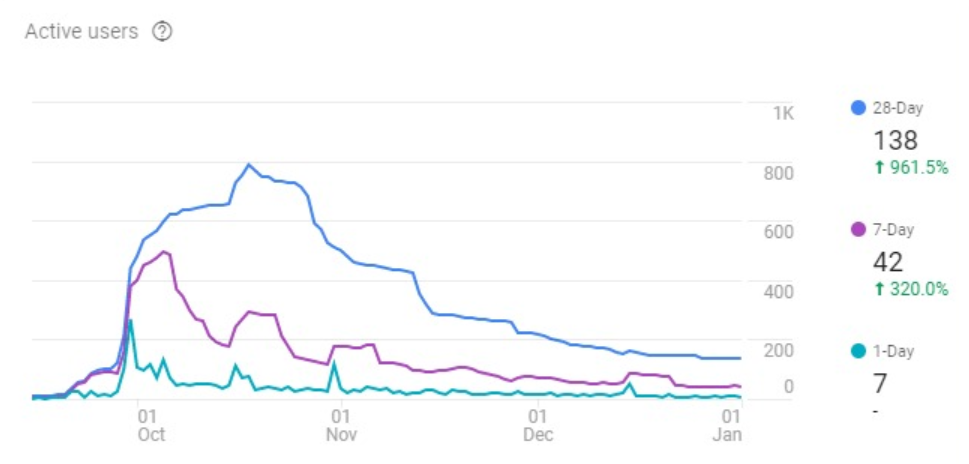
\includegraphics[width=0.89\textwidth]{figures/charts/politehnik_usage.png}
        \caption{Active users on the application \textit{Politehnik}, as reported by \textit{\gls{firebase}}}
        \label{2:fig:politehnik_usage}
    \end{figure}
    
    \subsection{Other tools} \label{2:existing_apps_other}
    Albeit not a mobile application, a relevant platform as far as \textit{tools made by students for students} go, is \textit{CTI Info}\footnote{https://infocti.github.io/}. It is a webpage made by a student in 2017, aiming to act as a small compendium with information that is particularly relevant for students pursuing the Computer Science domain (also known as CTI) within the faculty. This acts as a good example as to what kind of information our app should provide: it contains details about various platforms, student associations, a small FAQ section (including information about reading the timetable and a thoroughly explained campus map), as well as other useful resources.

\section{Mixing and matching for our application} \label{2:mix_and_match}

    % \subsection{Collaboration is key} \label{2:mix_and_match_collaboration}
    Since university apps (section \ref{2:uni_apps}) generally provide a lot of useful information (which may, however, sometimes be out of date) but lack customizability, while generic apps (section \ref{2:generic_apps}) are highly customizable but difficult to set up, we believe that a \textit{collaborative approach} would be the best middle ground.
    
    \acrshort{acs} students have a long history of putting materials together in order to help each other, be it through \textit{WhatsApp} or \textit{Facebook} groups, or through various websites\footnote{http://andrei.clubcisco.ro/, http://exams.ro/} or shared \textit{Google Drive} folders. Furthermore, thanks to our \textbf{\nameref{chapter3}}, we know that we can safely assume that there will always be at least one student who takes the time to thoroughly create events for themselves as they arise - we can take advantage of this and provide these students with a way to easily share the events with their colleagues. In the unlikely event that there is a group where not a single student naturally takes these notes, the task can fall to the group representative, or even better, all students in the group can contribute. However ideal that may seem on the surface, the implications are far-reaching: for starters, as seen on social media platforms nowadays (e.g. \textit{Facebook} groups, \textit{Reddit} subreddits), any platform where multiple people can collaborate requires a content moderation system\cite{roberts2019behind} to function reliably, a subject we will discuss more in section TODO.
    
    A collaborative system would also mean that we do not need to rely on a single person (such as the developer in the case of the app \textit{Politehnik}, described in subsection \ref{2:existing_apps_timetable}) or a small group of people (the app administration staff in the case of most official university applications, as seen in subsection \ref{2:uni_apps_case_study}) to keep the information relevand and up to date. As benefits of collaborative learnig have long been proven\cite{klemm1997benefits}, we could assume that, if enough users without malicious intent (further discussion in section TODO) contribute to a data set, customizability is intrinsic and data is unlikely to be inaccurate or out of date.
    
    % TODO Maybe move this section to another chapter further down
    
    % \subsection{Future improvements and integrations} \label{2:mix_and_match_future}
    % Since our ultimate goal is to help students, we do not see other published apps meant for students as competition, but rather as an opportunity to learn and improve our own application. We believe that building upon the existing technologies is better than trying to re-invent the wheel and create more confusion among students, who would have yet more tools for the exact same job.  Consequently, in the future, we aim to integrate with existing, published applications (e.g. \textit{UPBCampus}, described in section \ref{2:existing_apps_navigation}, and \textit{Politehnik}, described in section \ref{2:existing_apps_timetable}) in order to extend our app's functionality. Users can select certain options in our app and be redirected to another app that does what they are looking for, through URL schemes\footnote{https://developer.apple.com/documentation/uikit/inter-process\_communication} in iOS or the more well-rounded concept of Intents\footnote{https://developer.android.com/guide/components/intents-filters} on Android. Two possible integrations with the aforementioned tools would be, for instance, navigating to a location of an event saved in our application, by using the \textit{UPBCampus} app, or adding the \textit{Politehnik} events users are interested in into the calendar in our app.
    
    % Additionally, thanks to the students interviewed for our \textbf{Case study} (section \ref{2:uni_apps_case_study}) and the survey in our \textbf{User study} (chapter \ref{chapter3}), we can define additional features that would further improve the usefulness of our application, namely:
    % \begin{itemize}
    %     \item TODO
    % \end{itemize}
\chapter{User study} \label{chapter3}

Before designing the application, we needed to find out more about the needs and wants of students enrolled at \acrshort{acs} and the general context in which this application would function.

\section{Methods} \label{3:methods}

The research and data collection methods we used were \textbf{observation} (throughout the four years that the main author of the paper was enrolled at our faculty of choice, \acrshort{acs}), \textbf{interviews} (with students, professors as well as administrative personnel of the faculty) and a \textbf{survey}, the results of which we will be focusing on in this chapter.  We mention and discuss the results of the first two methods throughout the whole paper, where they offer insightful information for the specific section. Additionally, throughout every step of the whole process of designing the application, we went through a \textbf{feedback loop} with a small group of students to ensure that we were progressing in the right direction.

Partly due to the pandemic, the main method of communication with our potential users was online communication. Most of the interviews were done either via video call (through Microsoft Teams\footnote{https://teams.microsoft.com/}) or via chat (Facebook Messenger\footnote{https://messenger.com/}, WhatsApp\footnote{https://www.whatsapp.com/}) or e-mail (Gmail\footnote{http://gmail.com/}). The survey was a Google Form\footnote{http://forms.google.com/} shared both verbally and through social media platforms, receiving 212 responses between October and December 2019. Since we regrettably could not gather a relevant number of responses from Master's students, with only seven responses, we will be focusing on the Bachelor's students, since 200 out of the total of about 600 enrolled B.Sc. students is statistically relevant.

To analyze the data, we imported the results from the form into a database using Microsoft SQL Server\footnote{https://www.microsoft.com/en-us/sql-server/}, normalized the data and created visualizations using Microsoft Power BI\footnote{https://powerbi.microsoft.com/}.

\section{Target audience} \label{3:target_audience}

Studies\cite{hammer2011importance}\cite{connelly2013demographic} show that demographic information in surveys helps to avoid bias towards a specific section of the target audience. Therefore, we included some \textbf{demographic questions} to ensure that the pool of respondents is relatively balanced.

In terms of \textbf{gender demographics}, our results (fig. \ref{3:fig:gender}) closely match a separate study\cite{codette2019stats} that is specifically targeting gender demographics at computer science faculties in Romania, including \acrshort{acs}.

\begin{figure}[ht]
    \centering
         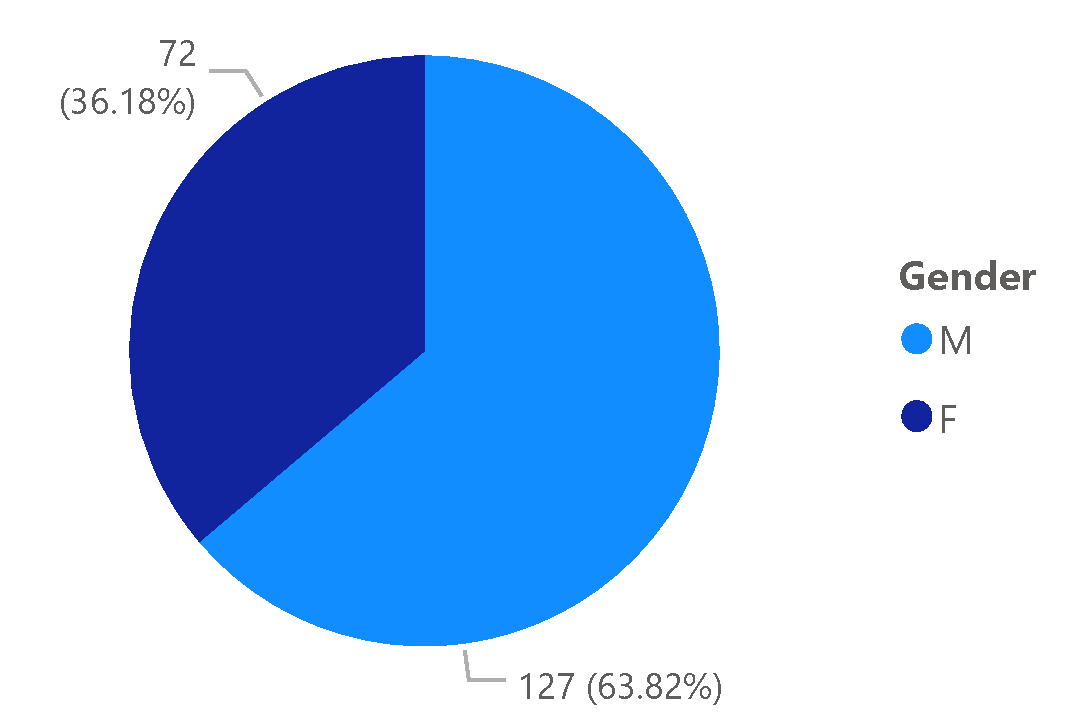
\includegraphics[height=0.2\textheight]{figures/charts/survey/gender.pdf}
    \caption{Gender of survey respondents}
    \label{3:fig:gender}
\end{figure}

Concerning \textbf{academic distribution}, we have received four times more responses from students pursuing the Computer Science domain (Computers and Information Technology, or CTI) than the Automatics domain (Systems Engineering, or IS), as seen in figure \ref{3:fig:domain}. Some discrepancy is expected, considering there are twice as many enrolled CTI students than IS students, according to the same study\cite{codette2019stats} mentioned above. The distribution of the respondents' year of study is relatively balanced (fig. \ref{3:fig:year}).

\begin{figure}[!ht]
    \centering
    \begin{minipage}[b]{0.49\textwidth}
        \captionsetup{justification=centering}
         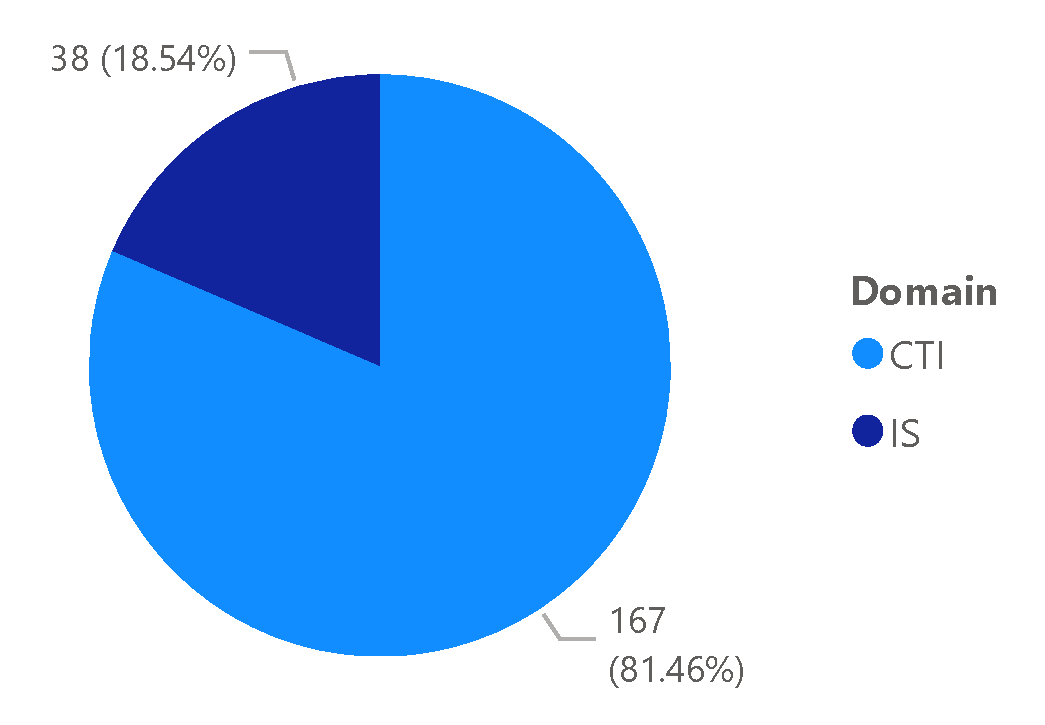
\includegraphics[height=0.2\textheight]{figures/charts/survey/domain.pdf}
        \caption{Domain of survey respondents}
        \label{3:fig:domain}
    \end{minipage}
    \hfill
    \begin{minipage}[b]{0.49\textwidth}
        \captionsetup{justification=centering}
         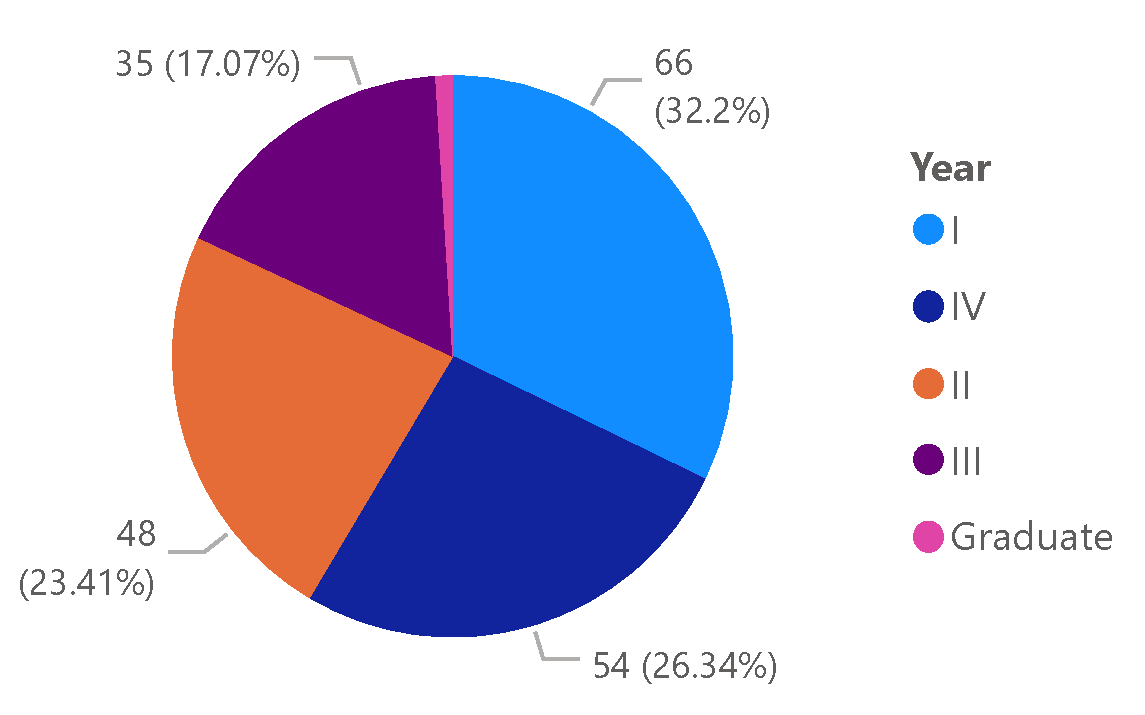
\includegraphics[height=0.2\textheight]{figures/charts/survey/year.pdf}
        \caption{Academic year of survey respondents}
        \label{3:fig:year}
    \end{minipage}
\end{figure}

Regarding \textbf{mobile operating systems}, the distribution is very similar to the Romanian mobile operating system market share, according to StatCounter GlobalStats \cite{statcounter2020mobile}, with 80\% of students using Android and 20\% of students using iOS.

\begin{figure}[ht]
    \centering
         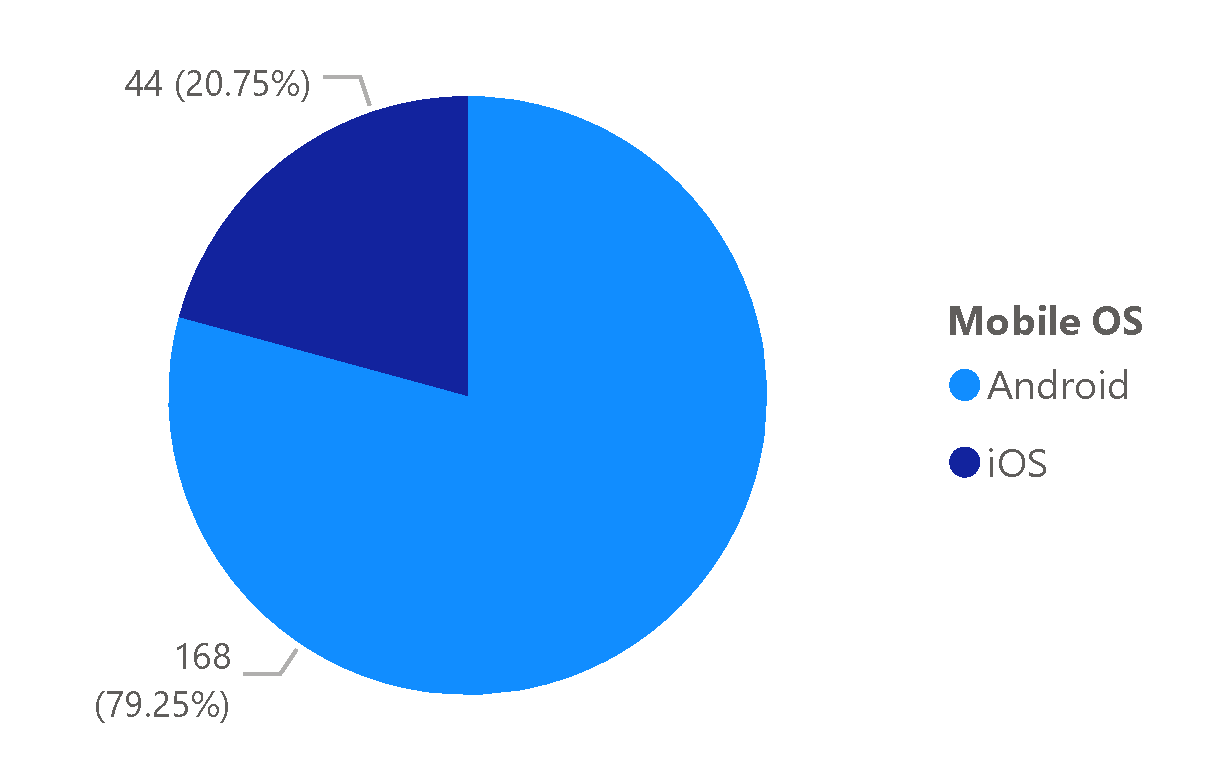
\includegraphics[height=0.2\textheight]{figures/charts/survey/os.pdf}
    \caption{Mobile \acrshort{os} of survey respondents}
    \label{3:fig:os}
\end{figure}

Upon reviewing the data, we believe that, aside from the lack of representation for Master's students, the respondents' demographics are varied enough for a relevant sample group.

\section{Results} \label{3:results}

We used a variety of questions to learn more about the student's preferences and what they would be looking for in a university mobile application. For this purpose, we included \textbf{multiple-choice questions}, \textbf{Likert scale questions} and \textbf{open-ended questions} in the survey.

\subsection{Features} \label{3:features}

The survey's primary purpose was to find out what kind of features would be the most useful for our students. We provided a list of potential features or types of information that could be available in the application and asked them to give each of them a rating from 1 (not very useful) to 5 (very useful). We devised a scoring system, with points between -2 and +3 for each answer, and came up with the hierarchy seen in figure \ref{3:fig:features}. The vast majority of students considered information and resources for classes and a timetable to be the most useful features.

\begin{figure}[ht]
    \centering
         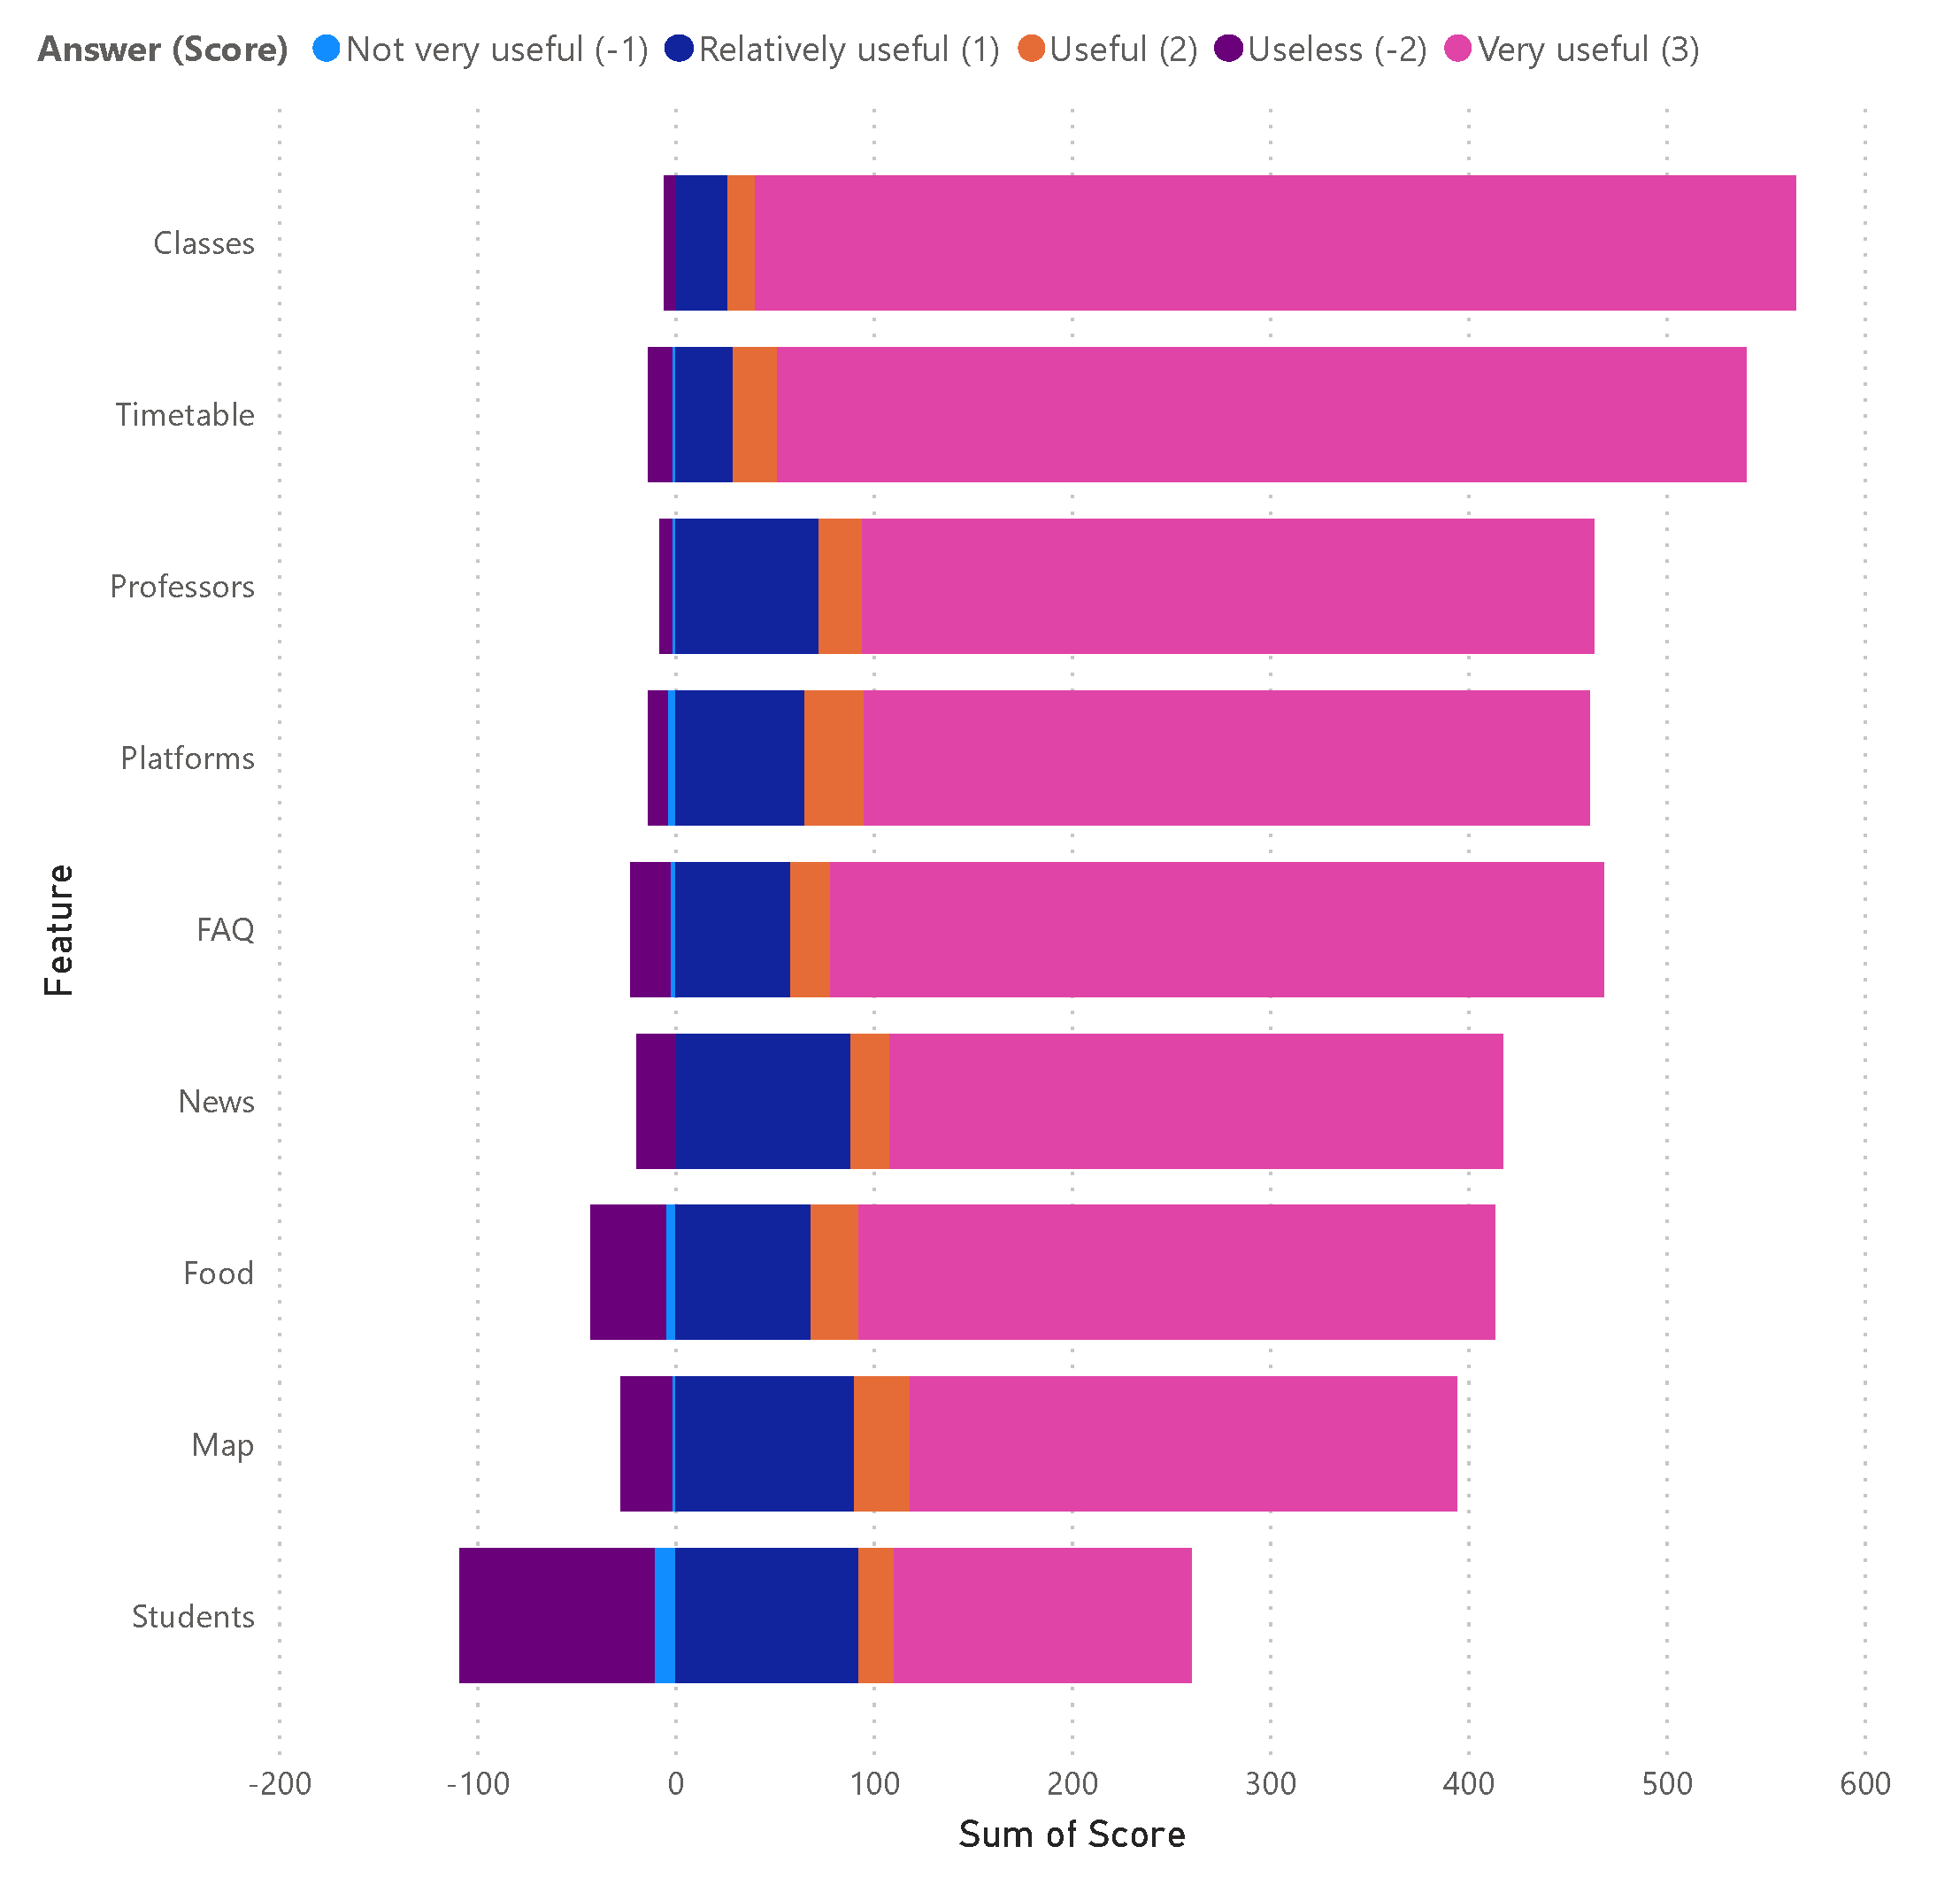
\includegraphics[height=0.57\textheight]{figures/charts/survey/features.pdf}
    \caption{Preferred app features for survey respondents}
    \label{3:fig:features}
\end{figure}

In an open-ended question, students suggested other features, such as an estimated waiting time for the canteens and a way to upload files for easy access. In terms of useful information that should be available in the app, some students suggested administrative information (about scholarships, or how to request specific documents) and feedback from other students about different classes and professors.

\subsection{Appearance} \label{3:appearance}

To find out how much we should prioritize coming up with an outstanding design for the application, we asked the students how important they believe the general appearance of an application to be. As seen in figure \ref{3:fig:appearance}, a vast majority of students believes appearance to be important or very important. Therefore, we need to focus as much as possible on the design step of the development process, described in chapter \ref{chapter4}.

\begin{figure}[ht]
    \centering
         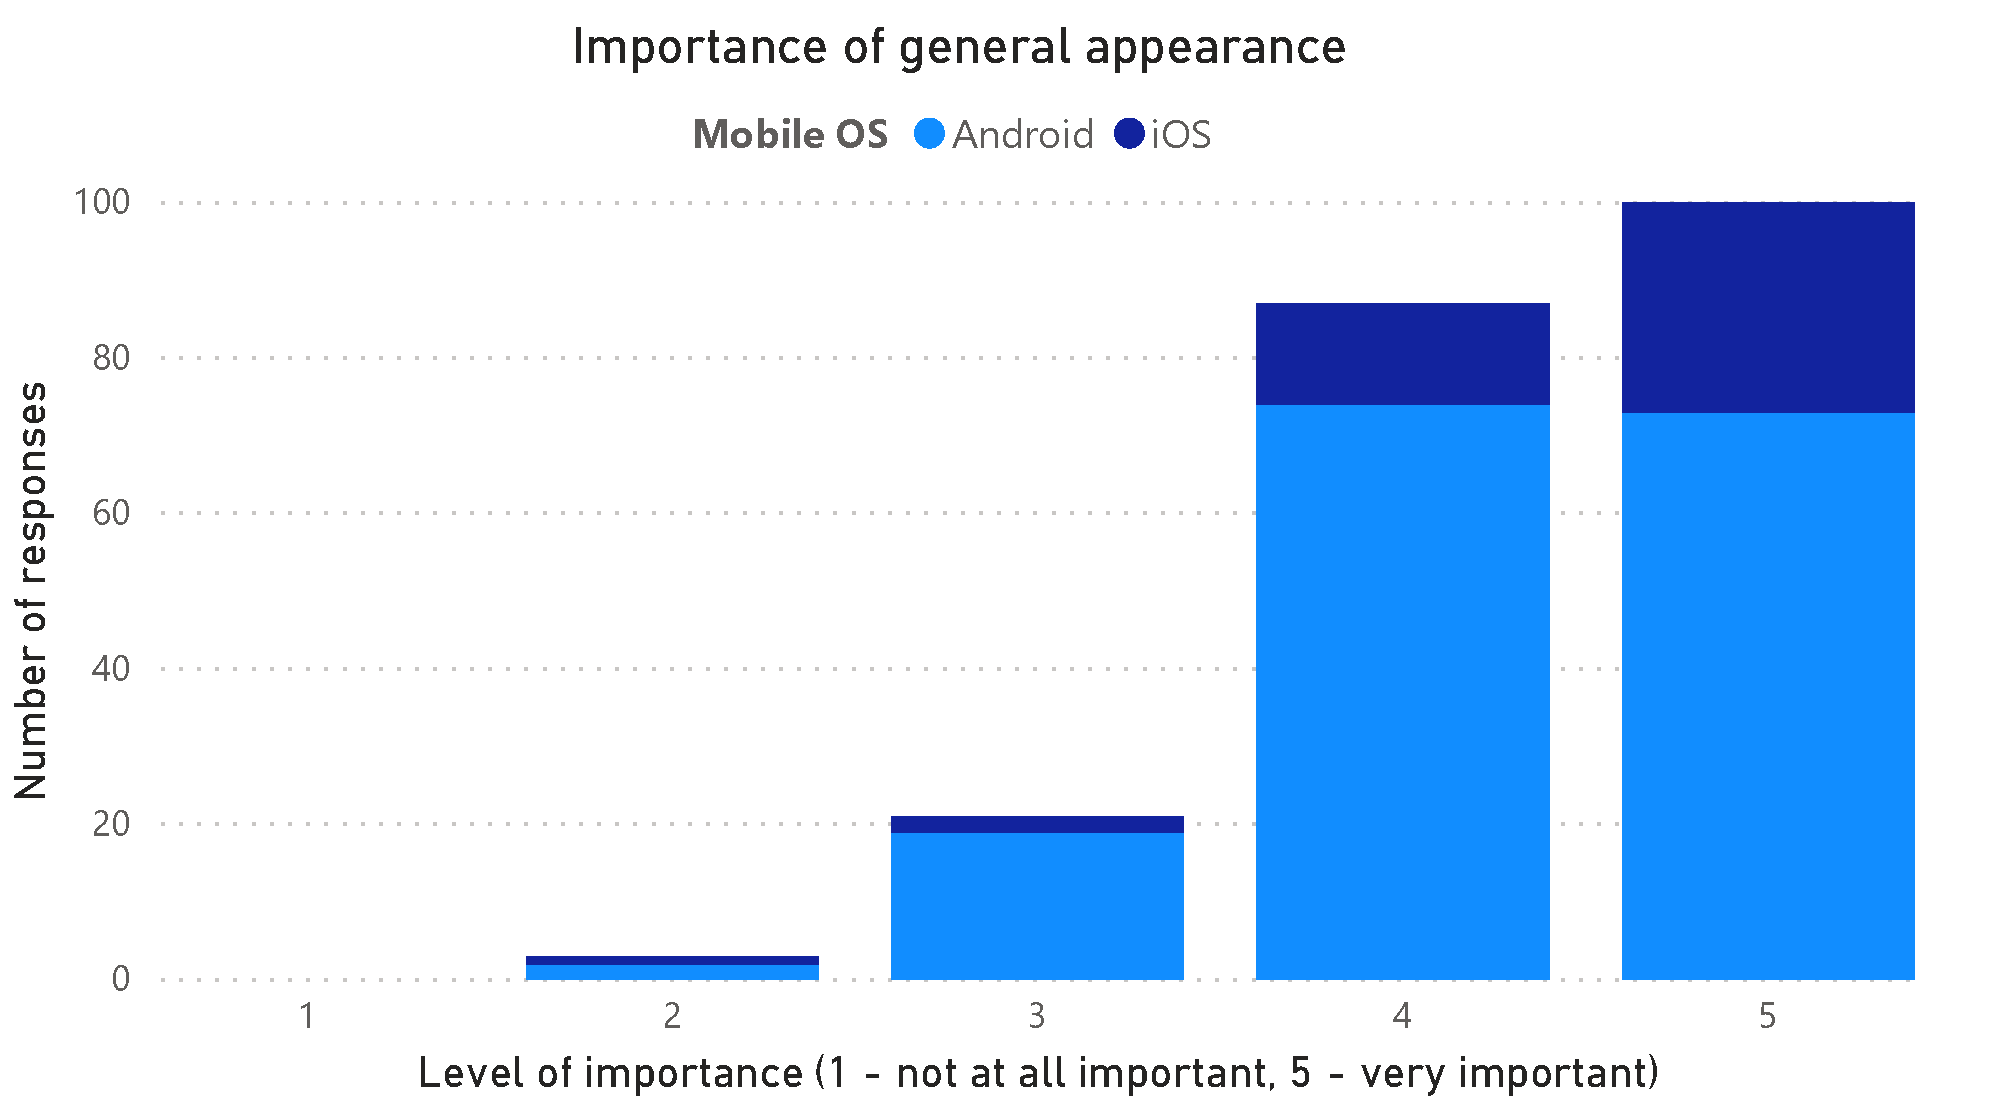
\includegraphics[width=\textwidth]{figures/charts/survey/appearance.pdf}
    \caption{Importance of general appearance by \acrshort{os} for survey respondents}
    \label{3:fig:appearance}
\end{figure}

In an open-ended question, several students stressed that performance, as well as how smoothly an application works, are also essential factors. Additionally, some students mentioned that they prefer a simple, easy to understand menu that doesn't require a user to go through more than three steps to achieve a specific goal. Through this, they were referencing the 3-click rule of web design (as defined by Catherine E. Weeks\cite{weeks1997design}, "A person shouldn't have to click more than 3 times to find a piece of info"). However, we will not be focusing specifically on this arbitrary \acrshort{ux} requirement, because multiple studies\cite{porter2003testing}\cite{nielsen2006prioritizing} have proved it to be nothing other than a myth.

One difficulty in designing a cross-platform application is that different platforms have different design guidelines that tend to be quite different\cite{thirumala2017interaction}. To help decide on a common design language for the application, we asked students how important native appearance is for them in a mobile application. We split the answers based on the student's mobile \acrshort{os} of choice, as seen in figure \ref{3:fig:native_appearance}. A native look and feel to an application is more important for iOS users than for Android users. However, it does not seem to be as important as the overall appearance of an application.

\begin{figure}[ht]
    \centering
         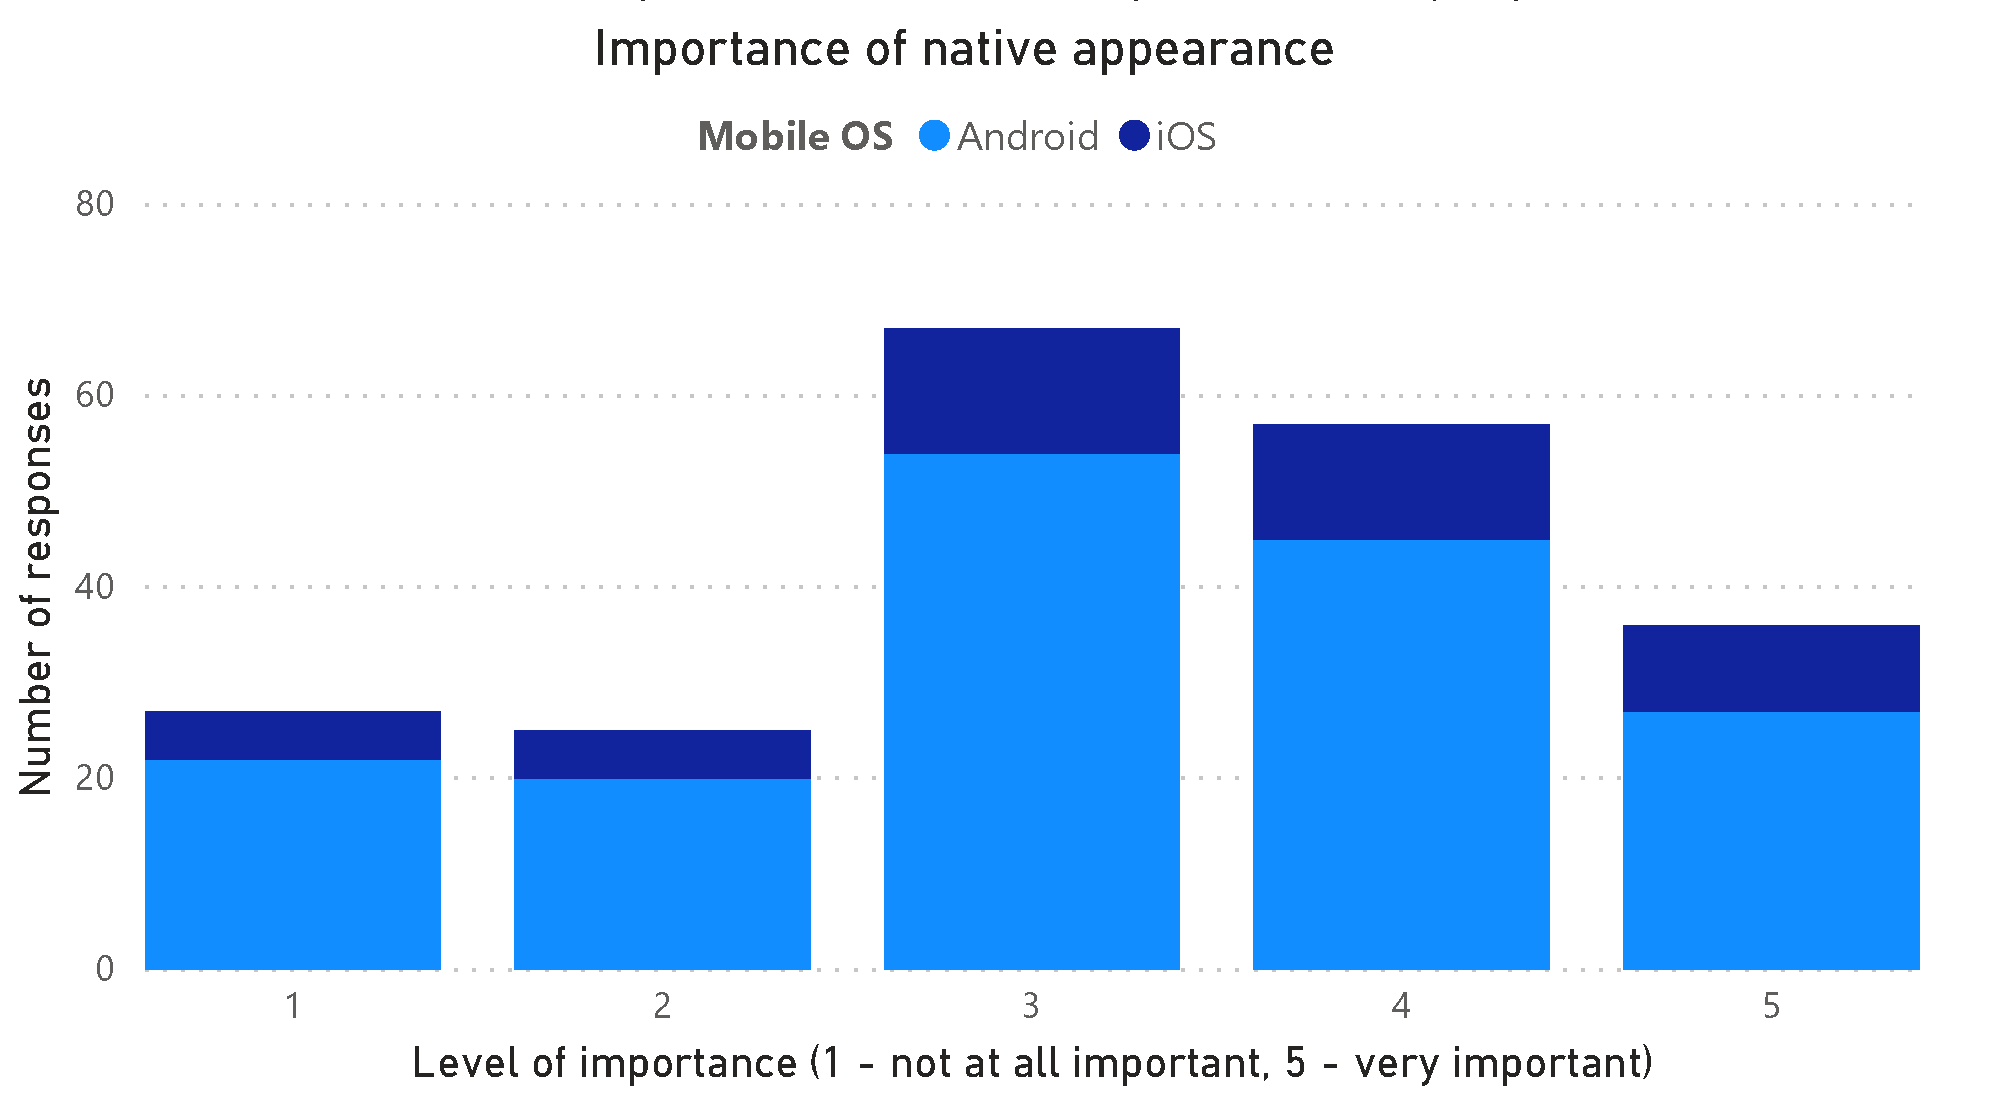
\includegraphics[width=\textwidth]{figures/charts/survey/native_appearance.pdf}
    \caption{Importance of native appearance by \acrshort{os} for survey respondents}
    \label{3:fig:native_appearance}
\end{figure}

Based on these results, we will attempt to come up with a smooth, intuitive interface that is based on but doesn't strictly abide by the design rules of either iOS (Human Interface Guidelines\cite{apple2020human}) or Android platforms (Material Design\cite{google2020material}). We will make it our goal to find a proper middle-ground solution for our cross-platform application.

\subsection{Language} \label{3:language}

Finally, we asked students what language they prefer their mobile \acrshort{os} to be in, to find out whether we should prioritize localization for our application. Somewhat surprisingly for a faculty with almost exclusively native Romanian students, more than half of respondents said that they prefer their mobile language to be English, as shown in figure \ref{3:fig:language}. Only 2\% of respondents chose a different answer, with only one student mentioning German and the others saying that they do not prefer one language over the other.

\begin{figure}[ht]
    \centering
         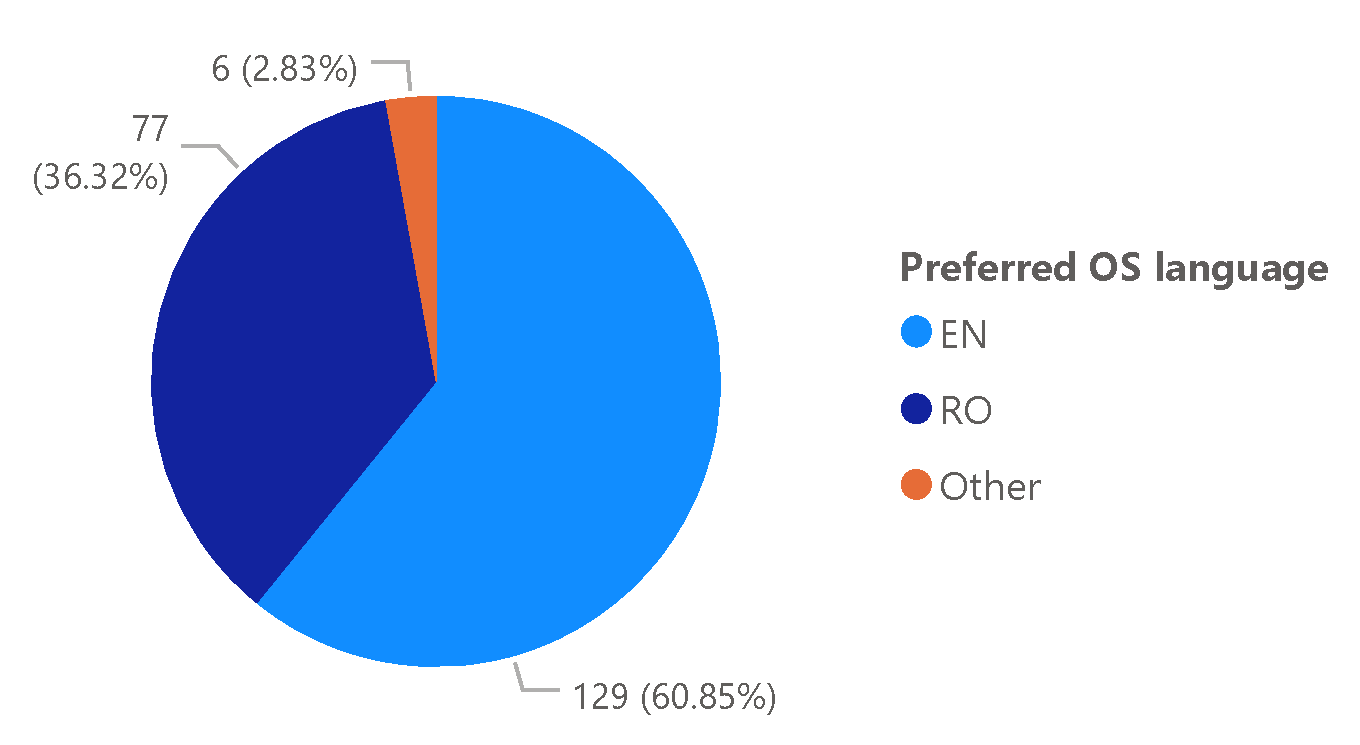
\includegraphics[height=0.2\textheight]{figures/charts/survey/language.pdf}
    \caption{Preferred \acrshort{os} language of survey respondents}
    \label{3:fig:language}
\end{figure}

With this data in mind, we know we need to pay close attention to our application's quality of localization. This feature is not just for the very few international students studying at \acrshort{acs}, but also for the many Romanian students who prefer their mobile devices and applications to be in English rather than their native language.
\chapter{\acrshort{ux} \& \acrshort{ui} design} \label{chapter4}

Because our survey indicated that we need to pay special attention to designing the interface of our application (see section \ref{3:appearance}), we decided to take an iterative approach to defining the \acrlong{ux} (\acrshort{ux}), and, by extension, sketching the \acrlong{ui} (\acrshort{ui}).

\section{Requirements} \label{4:requirements}

The proposed functionalities of our application are listed in section \ref{1:functionalities}. We will aim to reach our goals, as described in section \ref{1:goals}.

We will be designing a collaborative application (a decision motivated in section \ref{2:mix_and_match}) with a moderation system based on permission levels, described in this chapter in section \ref{4:permissions}.

Based on the results of our survey (section \ref{3:appearance}), our design language of choice will be neither Google's Material Design\cite{google2020material}, nor Apple's Human Interface Guidelines\cite{apple2020human}, but rather what we consider to be a healthy mix of both. This design aims to be pleasant for both Android and iOS users, as is required of a cross-platform application which aims to have a consistent design on all platforms. A good example of another such application is \textit{Reddit} (available on both the App Store\footnote{https://apps.apple.com/us/app/reddit/id1064216828} and Google Play\footnote{https://play.google.com/store/apps/details?id=com.reddit.frontpage} with a very similar design that only slightly differs in the web version\footnote{http://reddit.com/}). However, since it sports a platform-agnostic design, independent developers have come up with separate applications for viewing \textit{Reddit} content on Android and iOS devices, which claim to have a more "native" look for the more nitpicky users. A visual comparison between these applications can be seen in appendix \ref{a:native_cross}.

\section{Paper prototyping} \label{4:paper}

\subsection{Initial concept} \label{4:paper_concept}

We kick-started the design process by making a rough sketch of what we imagined the app to look like, on paper, with the features we had in mind in the beginning. We used the \textit{School Assistant} app (see section \ref{2:generic_apps}) as the main inspiration for this first design.

\begin{figure}[ht]
    \centering
         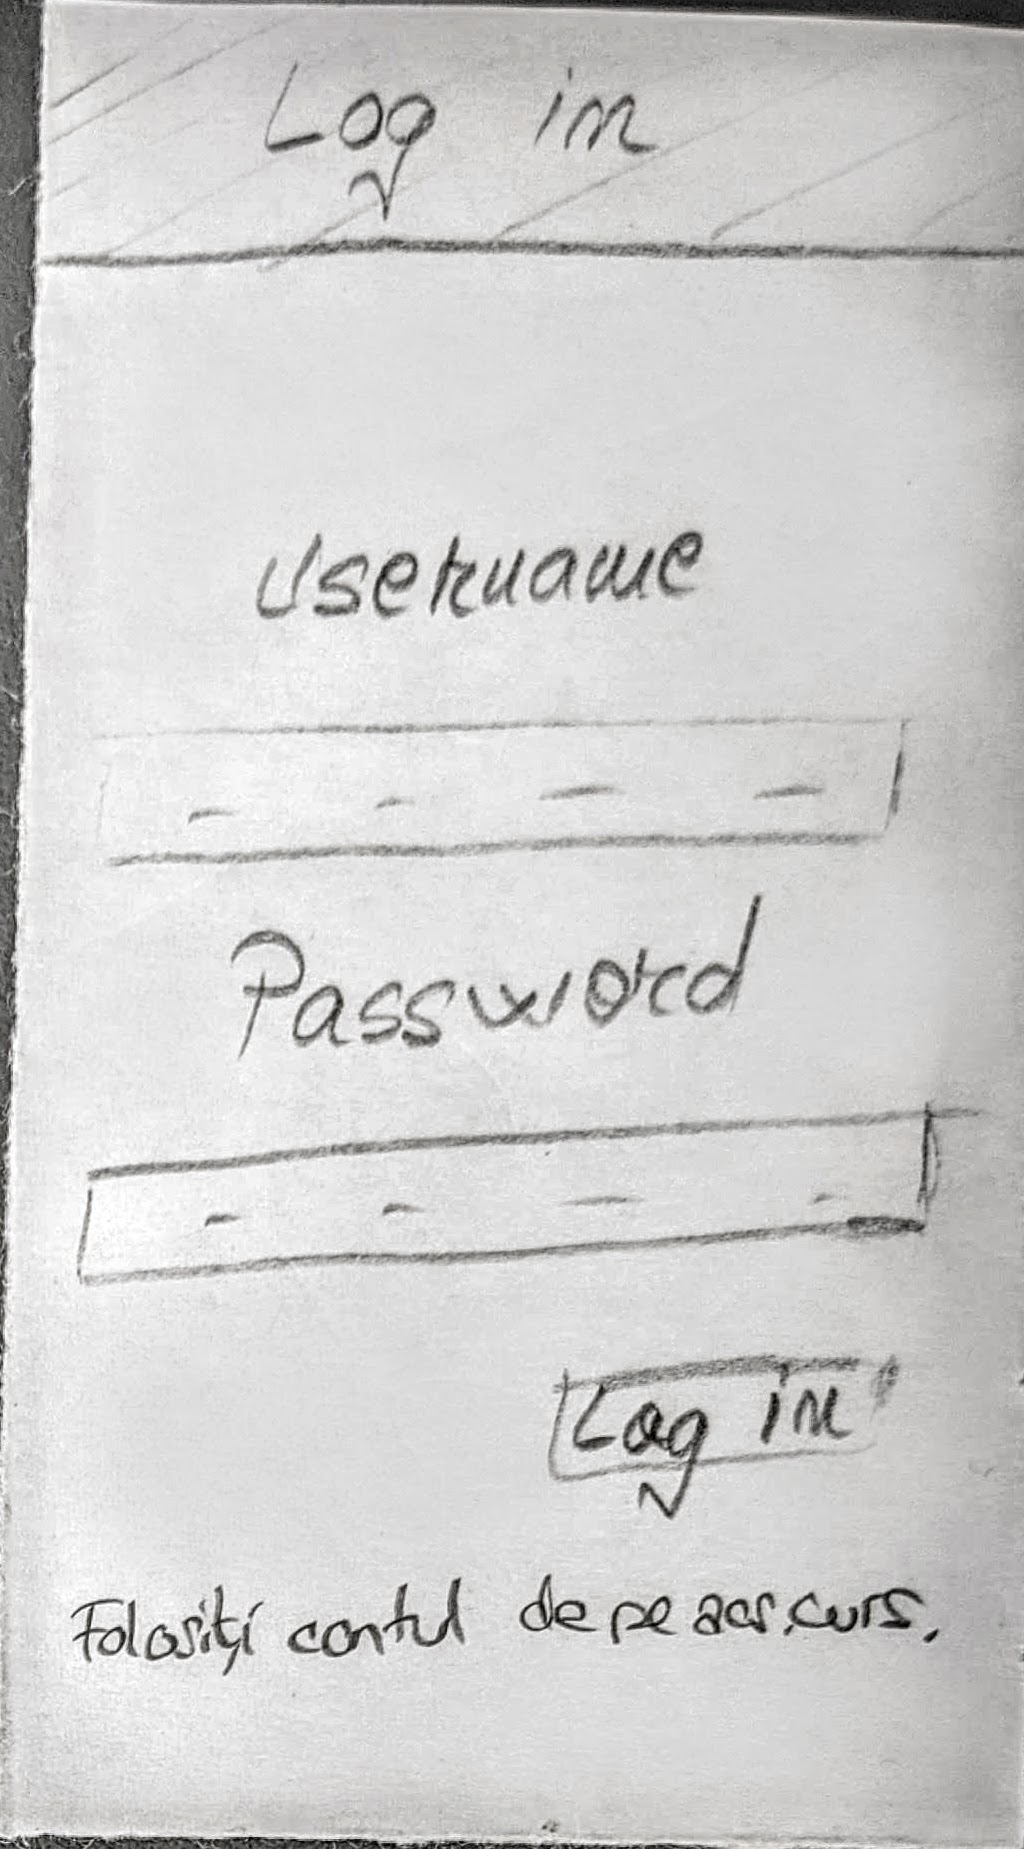
\includegraphics[height=0.279\textheight]{figures/app/paper/login.jpg}
         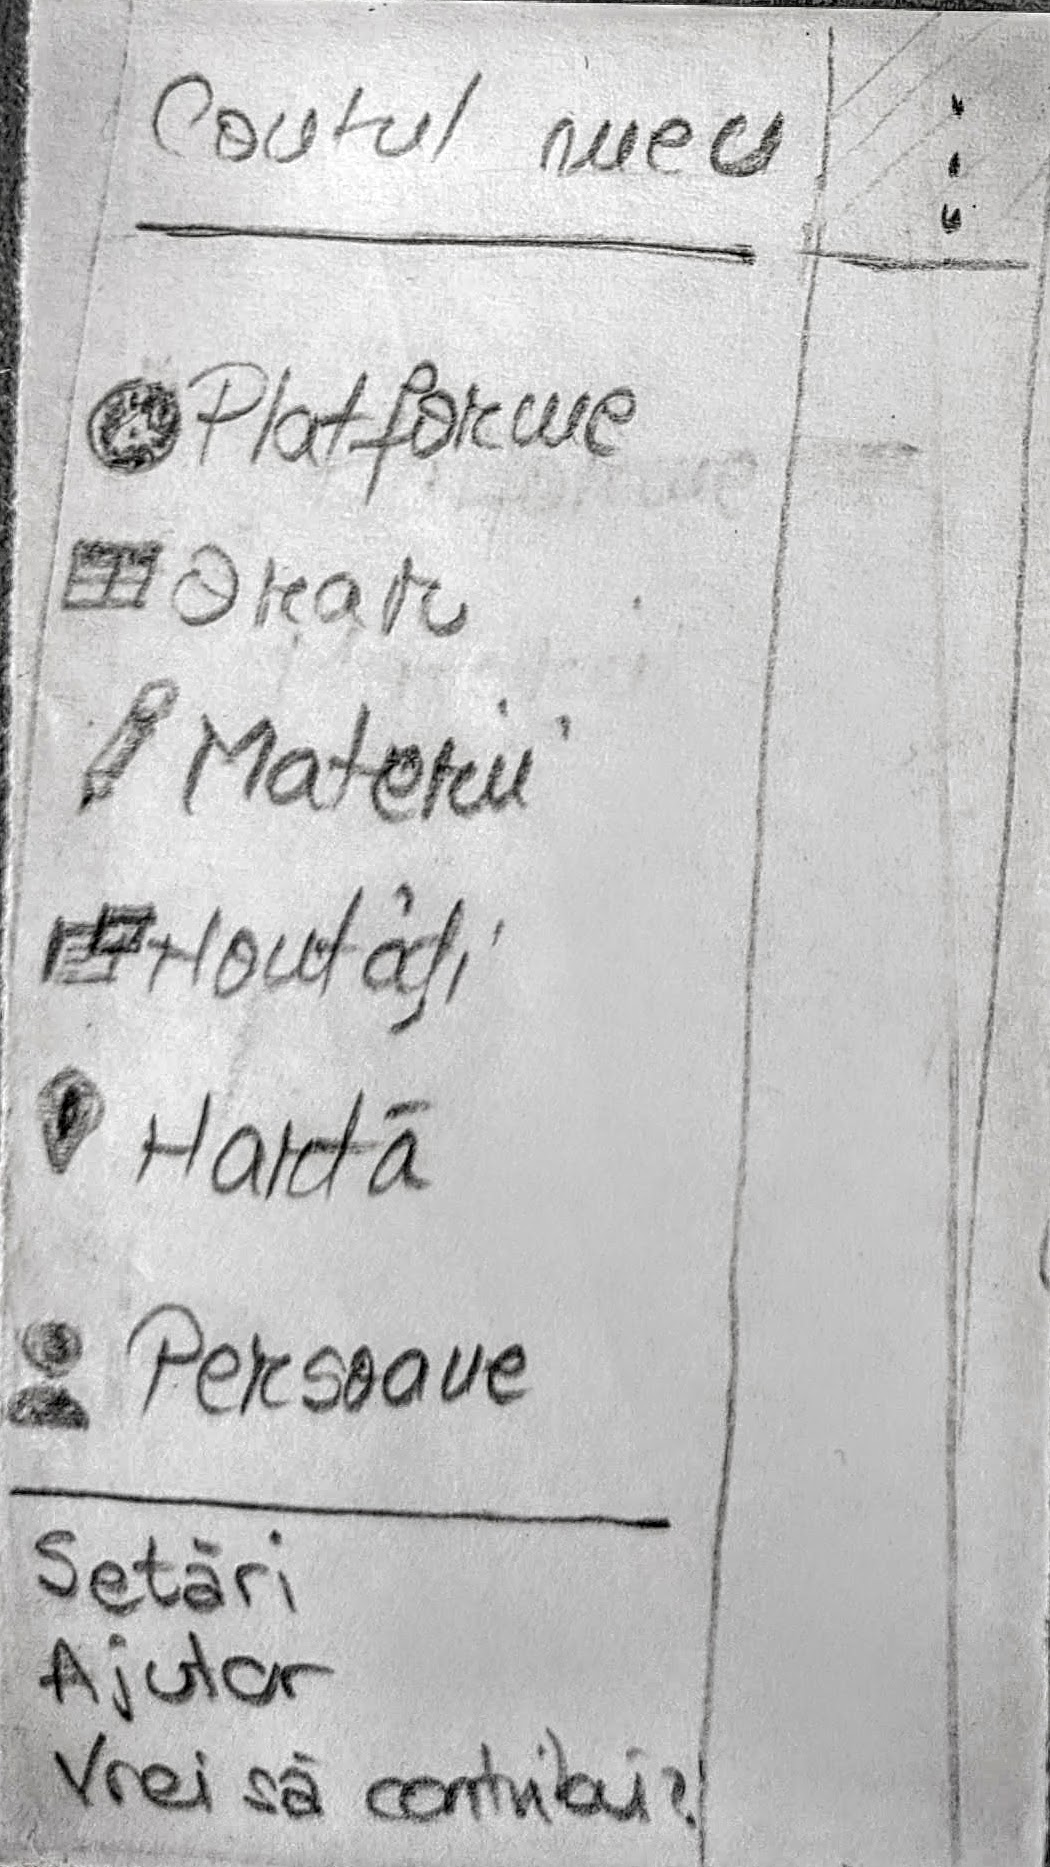
\includegraphics[height=0.279\textheight]{figures/app/paper/drawer.jpg}
         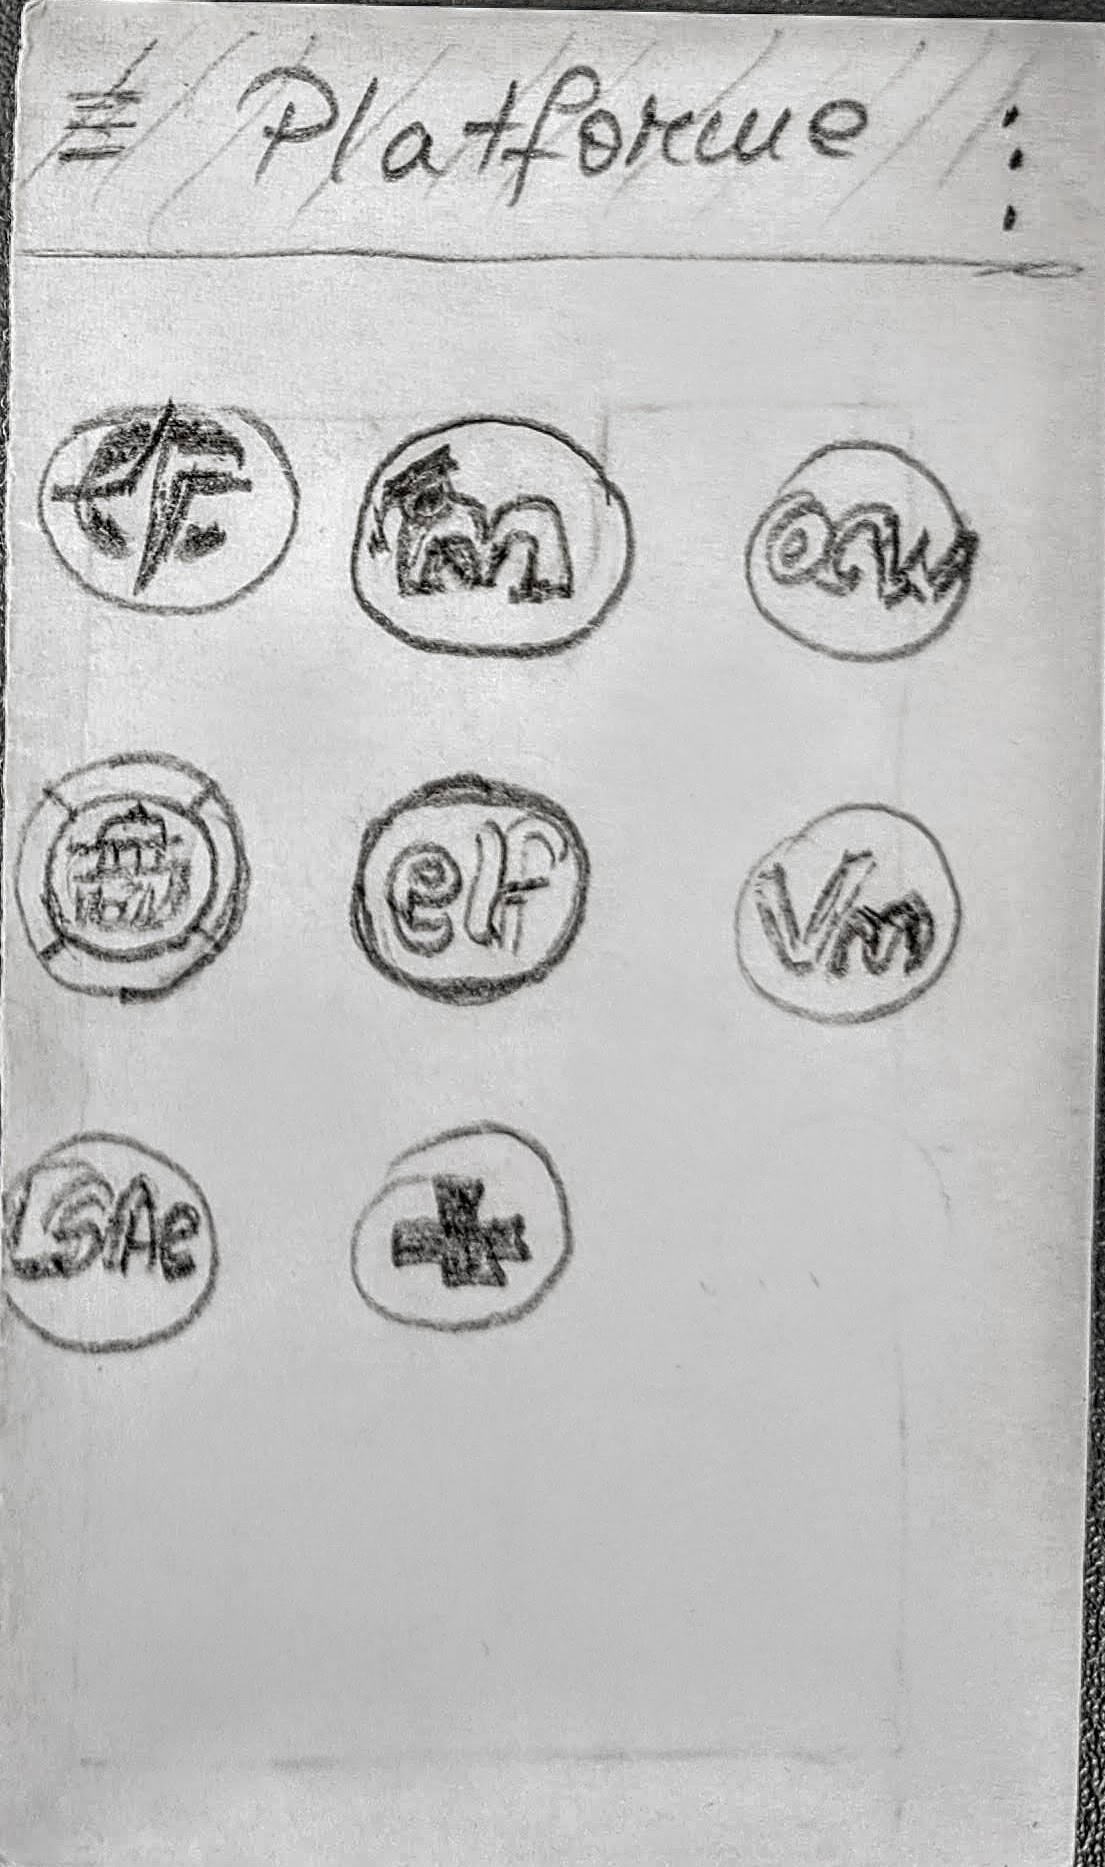
\includegraphics[height=0.279\textheight]{figures/app/paper/platforms.jpg}
         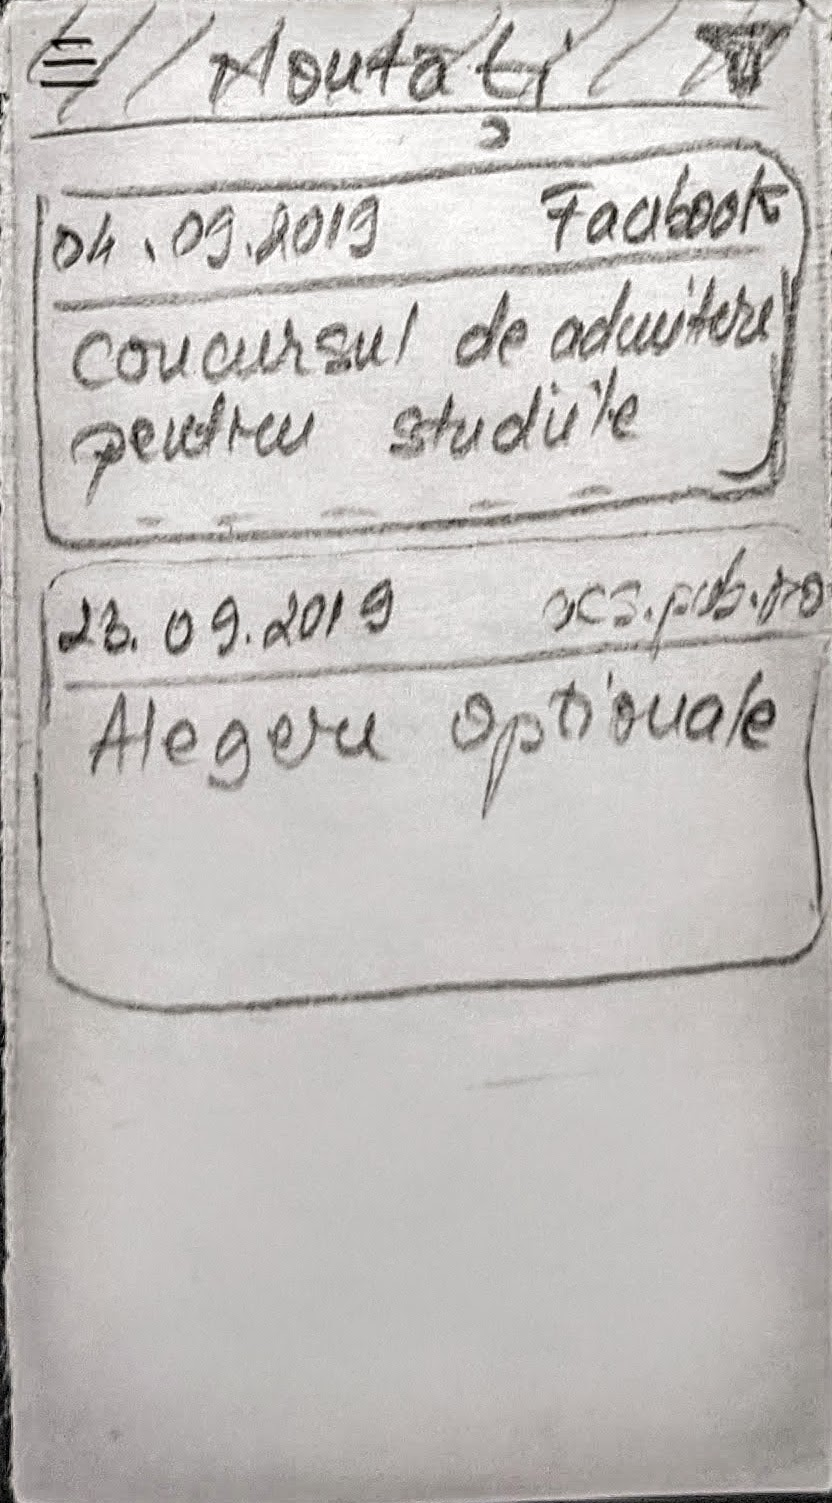
\includegraphics[height=0.279\textheight]{figures/app/paper/news.jpg}
         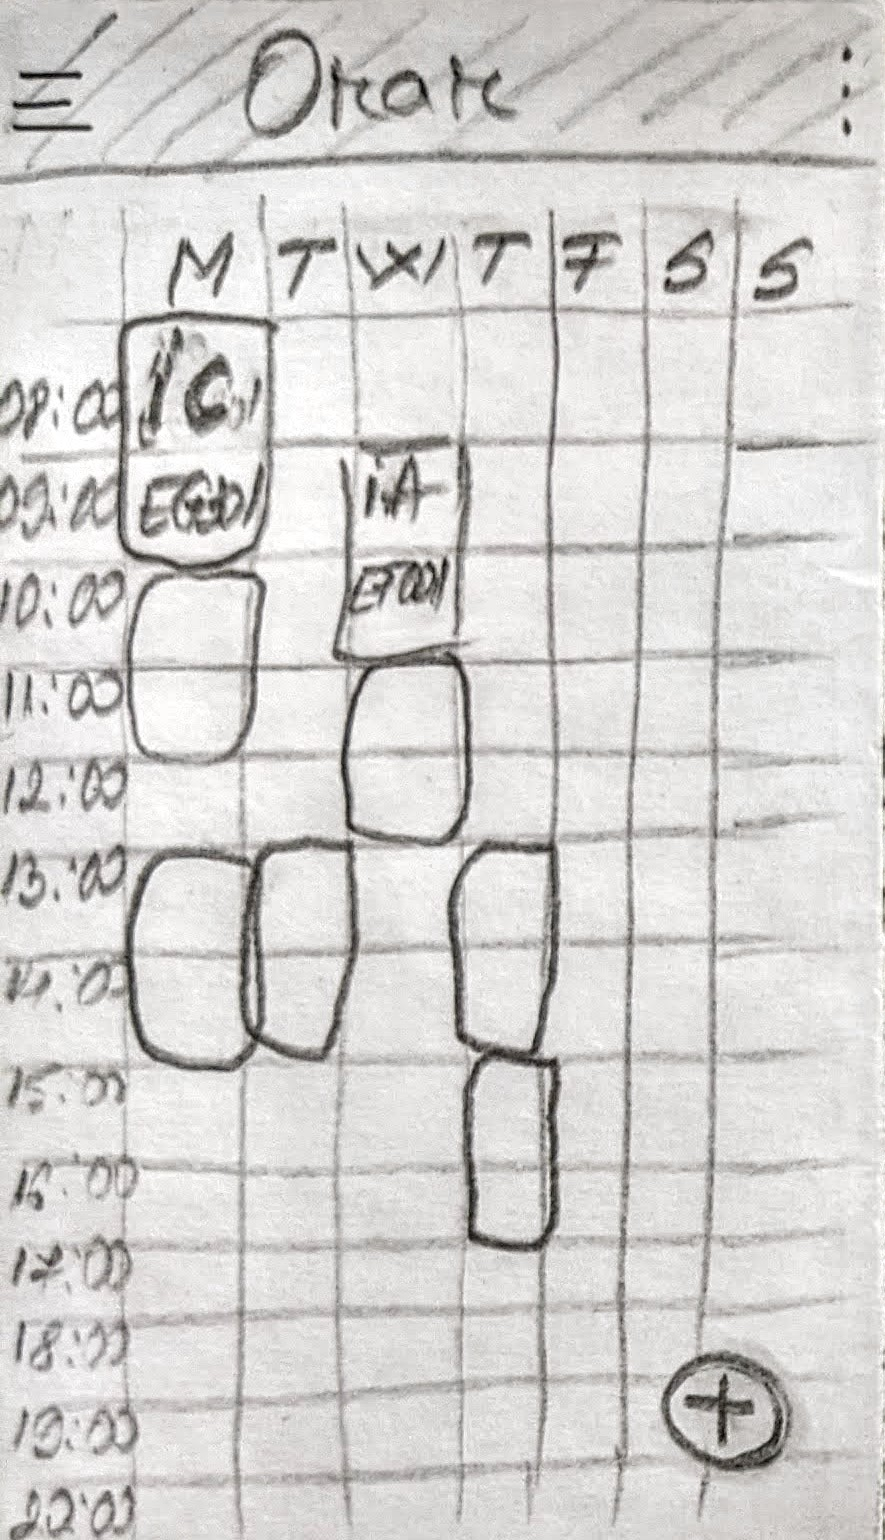
\includegraphics[height=0.279\textheight]{figures/app/paper/timetable.jpg}
         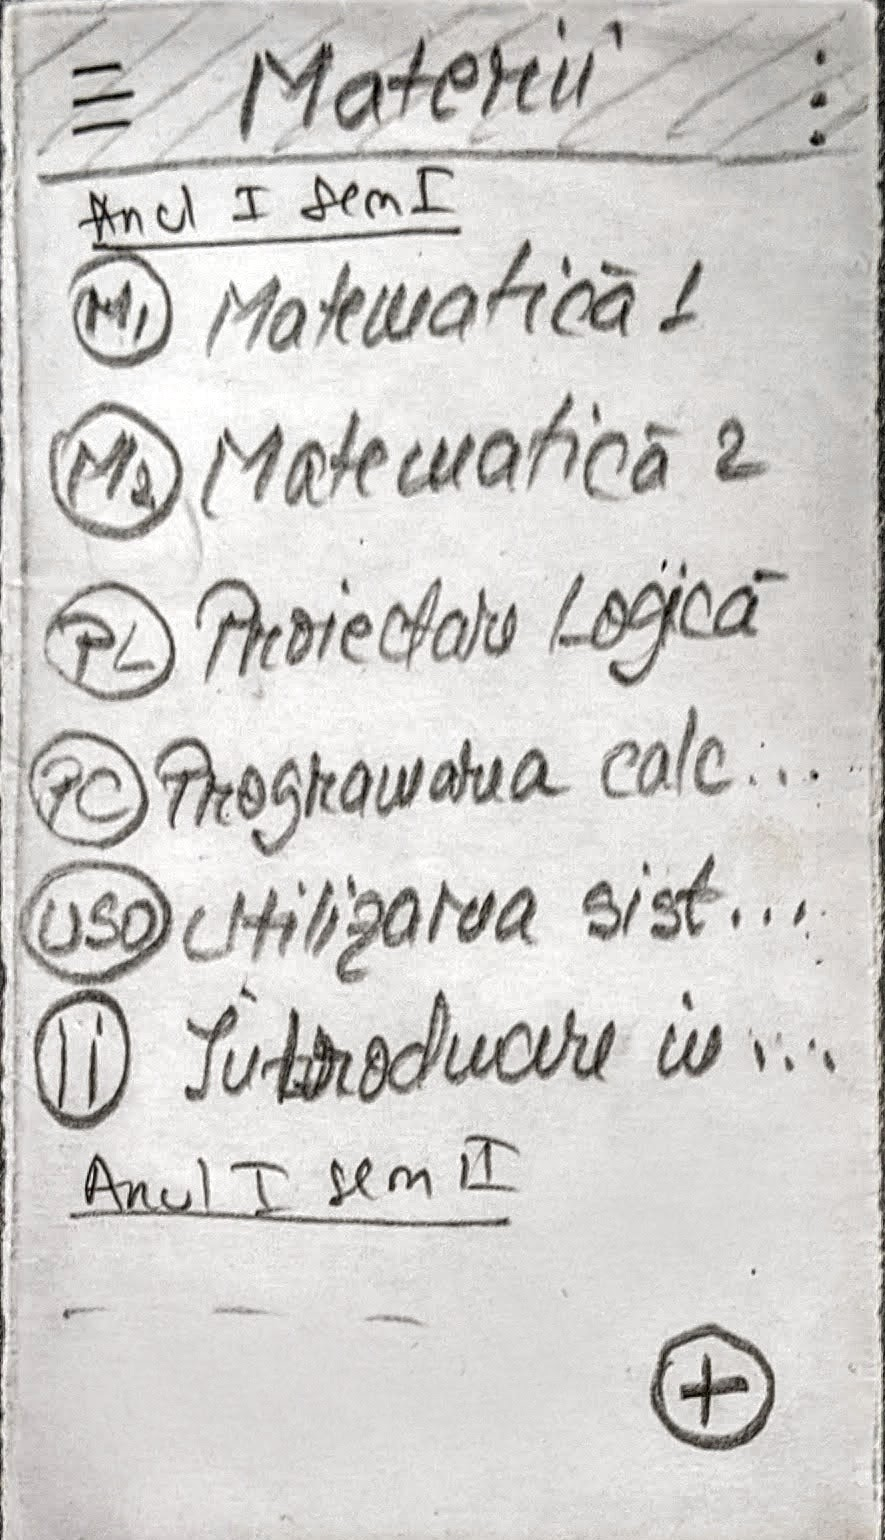
\includegraphics[height=0.279\textheight]{figures/app/paper/classes.jpg}
         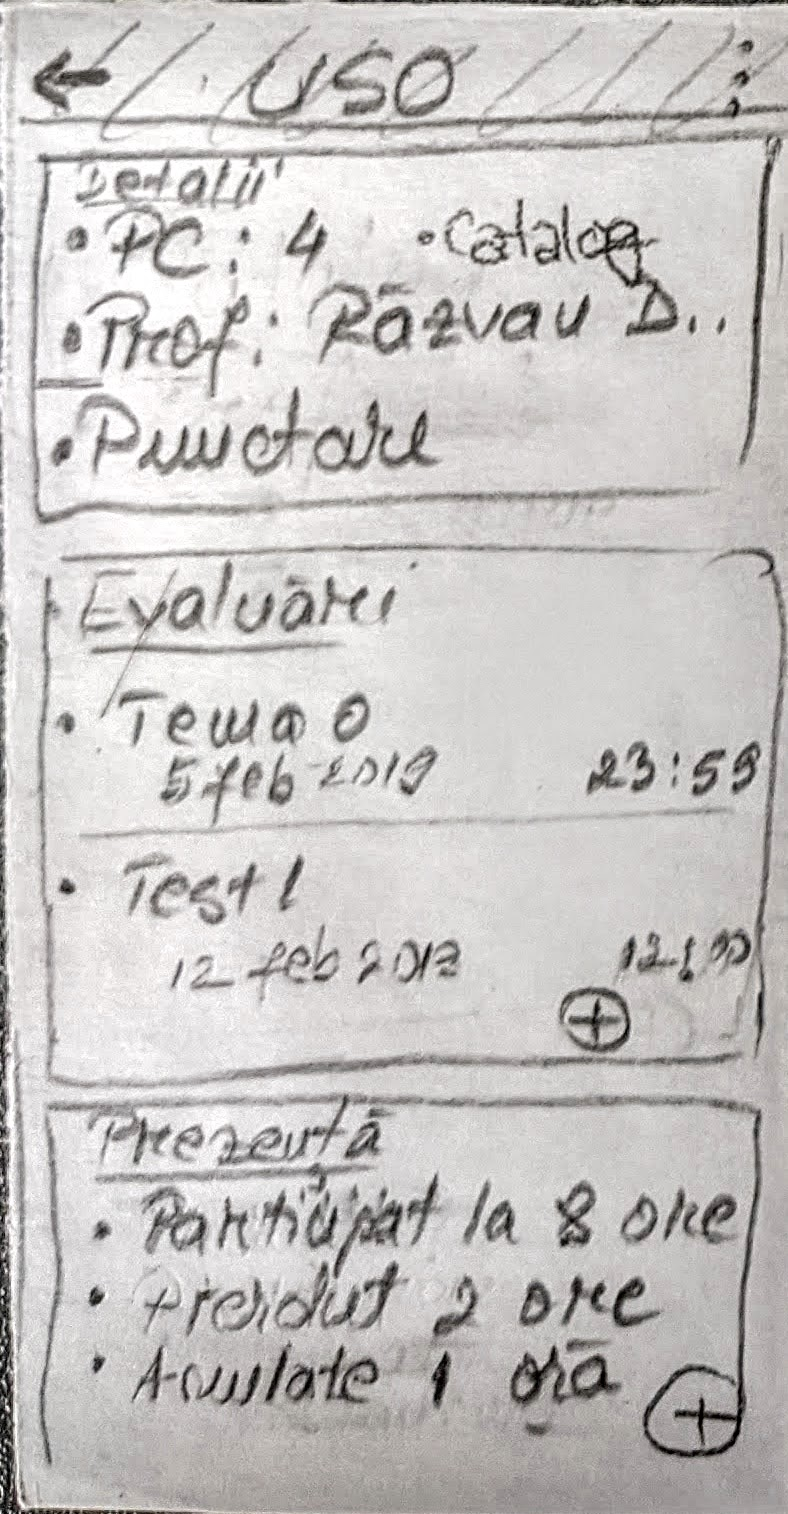
\includegraphics[height=0.279\textheight]{figures/app/paper/class_info.jpg}
         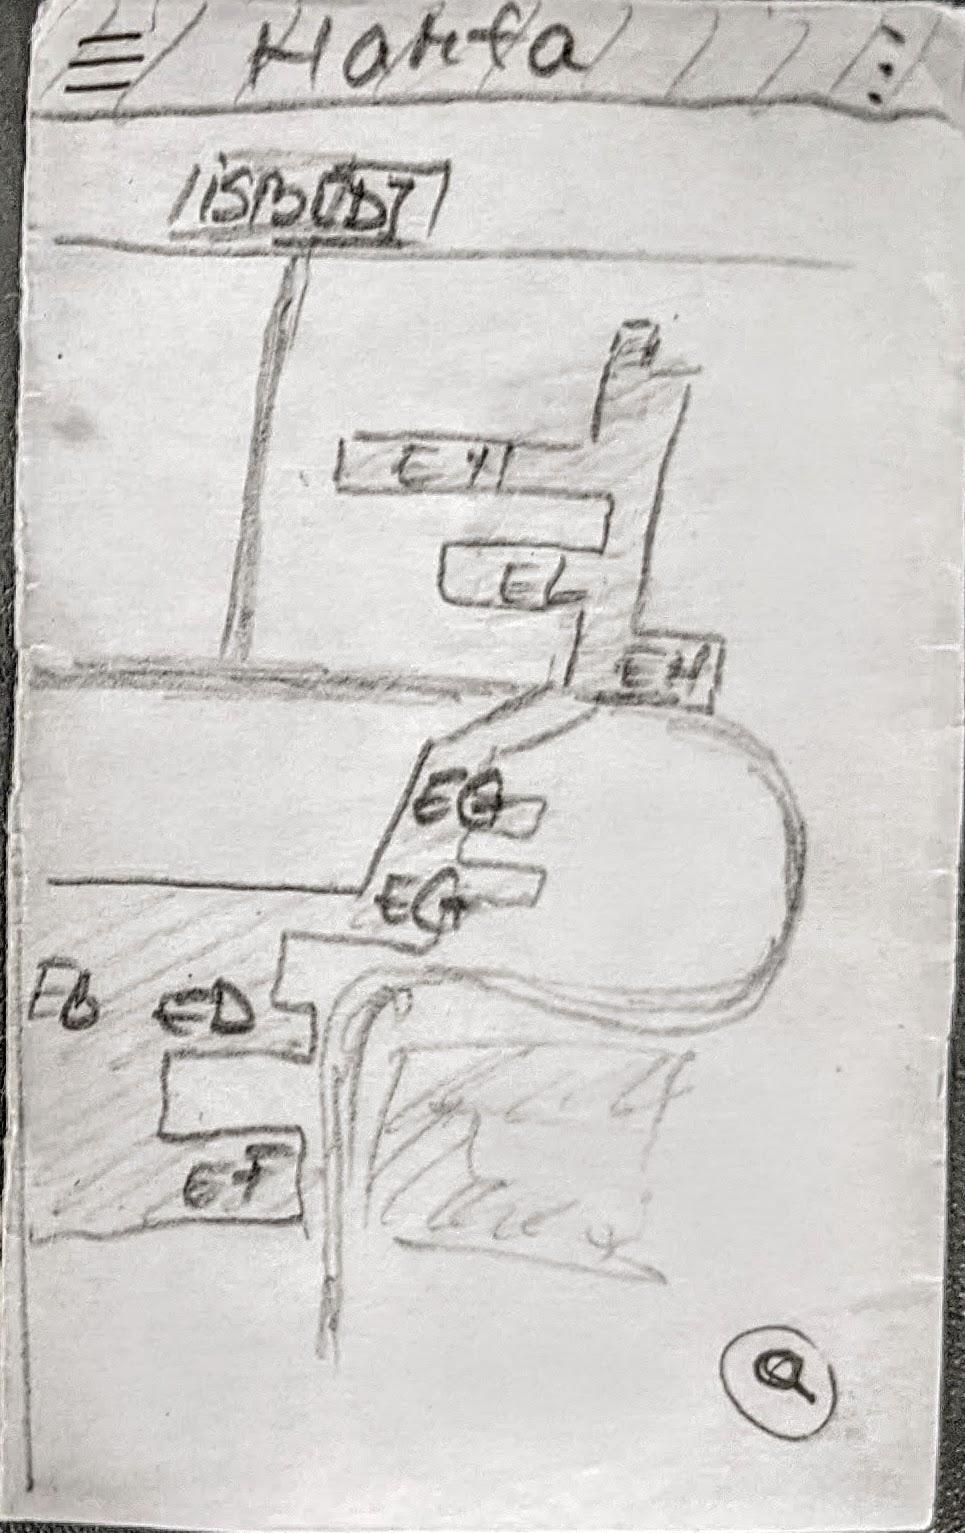
\includegraphics[height=0.279\textheight]{figures/app/paper/map.jpg}
    \caption{Paper prototype}
    \label{4:fig:paper_prototyping}
\end{figure}

\clearpage

Figure \ref{4:fig:paper_prototyping} shows the very first sketches of the application interface. The pages pictured, from left to right and top to bottom, are:
\begin{itemize}
    \setlength{\topsep}{0.5pt}
    \setlength{\itemsep}{0.5pt}
    \setlength{\parsep}{0.5pt}
    \item the login page the user would see when first opening the app
    \item the Material\cite{google2020material}-style side drawer with the different pages in the app, available once the user logs in
    \item a list of the university's platforms, which would serve as the default page the user would see without accessing the drawer
    \item the "News" page with information from various sources, such as relevant Facebook pages and the official website
    \item the timetable, with a button to add a new event
    \item the list of classes, organized by year/semester, with a button to add a new class
    \item information about a class that a user would see when clicking on an event or class
    \item the map of the campus, with a button to search for a specific location
\end{itemize}

\subsection{Feedback} \label{4:paper_feedback}

To find out what students would think about this initial concept, we organized a focus group with about 15 students and presented each of them the workflow of our application. Regarding \textbf{authentication}, we have received feedback regarding the need for a profile page for the user. The possibility for a user to use the app without having to authenticate was also mentioned. Multiple students pointed out that having the "Platforms" page as the default was counter-intuitive, and that a \textbf{designated "Home" page} would be a better solution. When asked what they think this homepage should contain, they suggested quick actions and upcoming events; in other words, an overview at a glance of the other pages within the app.

Some students pointed out that the homework-type events should have both \textbf{a soft and a hard deadline} associated with them, as is the norm in the faculty. Additionally, they wanted to see how the process of adding a new event would work.

\section{Permissions \& moderation system} \label{4:permissions}

\subsection{The need for moderation} \label{4:permissions_need}

As mentioned in section \ref{2:mix_and_match}, any collaborative system involving more than a few users requires some form of moderation\cite{roberts2019behind}. This system is meant to ensure that content stays accurate and up-to-date and avoid offensive/inappropriate content.

Based on the categories described by a \textit{Bridged.co} writer\cite{bridged2019moderation}, we will be using a mixture of \textbf{pre-moderation} and \textbf{reactive moderation}, meaning that content will be verified before appearing on the platform, and users can report or flag content that they believe to be inappropriate after it has been posted.

Since the platform should eventually be self-sustainable, without the need of constant involvement from the developer in content moderation (as is the case for the nonscalable solution of the application \textit{Politehnik}, described in section \ref{2:existing_apps_timetable}), we need a way to offer students the ability to moderate content on the platform themselves. This situation begs the question - how do we decide who should have the right to moderate content, and who should not?

\subsection{Permission levels} \label{4:permissions_levels}

To establish who should have certain rights, we need to define the rights that are to be granted. We have designed a permission-level system, where each user has a permission number, which indicates what they can do within the application. Each level includes the permissions of lower levels.

\begin{itemize}
    \setlength{\topsep}{0.5pt}
    \setlength{\itemsep}{0.5pt}
    \setlength{\parsep}{0.5pt}
    \item \textbf{0} - no special permissions; user can read public (already filtered) content and add private content or make suggestions
    \item \textbf{1} - helper level; user can view suggestions made by other people and vote up/down depending on whether they believe the suggestion to be appropriate or not
    \item \textbf{2} - basic moderator level; user can approve suggestions (an approved suggestion would be made public) and post content directly (without needing review); they can only delete content they posted or approved
    \item \textbf{3} - complete moderator level; user can dismiss suggestions (dismissed suggestions would be deleted from the suggestions page and no longer visible to anyone) and delete content added by anyone
    \item \textbf{4} - administrator level; user can change other users' permission level
\end{itemize}

\subsection{Assigning permissions} \label{4:permissions_assigning}

By default, any new user would have the first permission level (0). Initially, only the developers would have level 4, allowing them to assign special permissions to trusted students in their circle. Additionally, students who have a special status within the faculty (group/series representatives, certain members of student associations) can request to be granted level 2 to inform their fellow students easily.

In the future, a manually-defined permission system might prove not to be scalable. In this case, one potential solution would be for users' permissions to gradually increase as they contribute quality content to the platform (e.g., make/vote up suggestions that end up being approved, vote down suggestions that end up being dismissed). This system could be implemented into the application in a \textbf{gamified} manner (e.g., unlocking achievements and earning points by doing specific actions). Game-like platforms have a history of motivating students to participate actively. One such example within the faculty is \textit{World of USO}\footnote{https://wouso.cs.pub.ro/}, a competitive knowledge game played throughout the first semester by first-year students for the Introduction to Operating Systems (USO) class.

\section{Wireframe} \label{4:wireframe}

\subsection{Prototype} \label{4:wireframe_prototype}

Following the focus group, we noted the feedback and created a more detailed, interactive (clickable) wireframe using Balsamiq\footnote{https://balsamiq.com/}. We re-drew the login page (fig. \ref{4:fig:balsamiq_login}), drawer (fig. \ref{4:fig:balsamiq_menu}) and websites page (fig. \ref{4:fig:balsamiq_websites}), and introduced a home page (fig. \ref{4:fig:balsamiq_home}), as suggested by the feedback described in section \ref{4:paper_feedback}. The latter includes a list of frequently accessed websites, as well as upcoming events and tasks.

\begin{figure}[!ht]
    \centering
    \begin{minipage}[b]{0.25\textwidth}
        \captionsetup{justification=centering}
        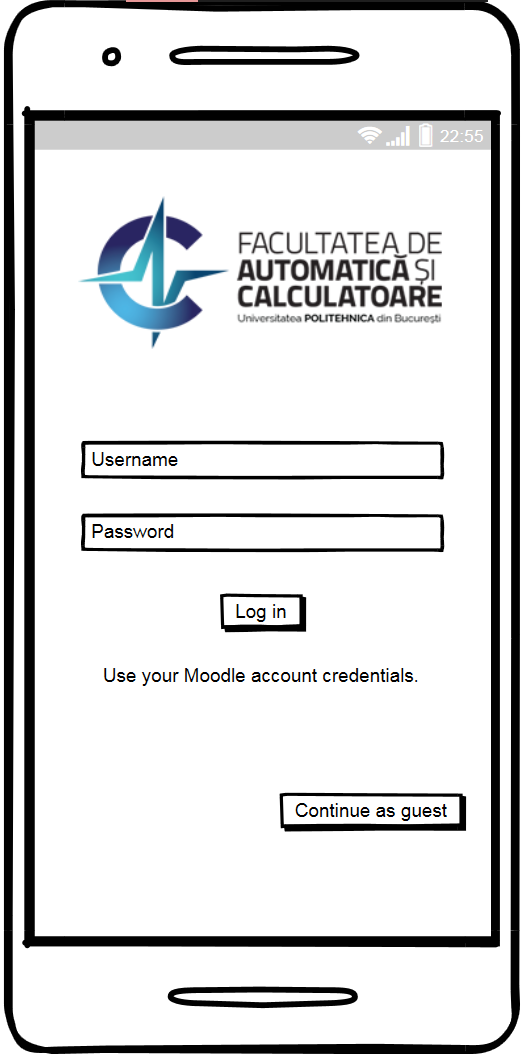
\includegraphics[width=\textwidth]{figures/app/balsamiq/login.png}
        \caption{Login page wireframe}
        \label{4:fig:balsamiq_login}
    \end{minipage}
    \hfill
    \begin{minipage}[b]{0.26\textwidth}
        \captionsetup{justification=centering}
        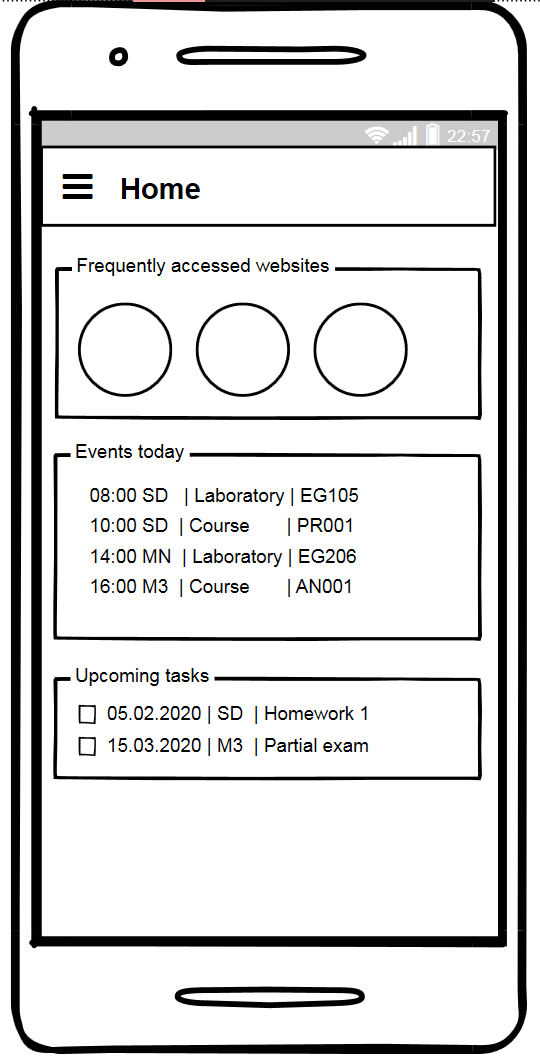
\includegraphics[width=\textwidth]{figures/app/balsamiq/home.png}
        \caption{Home page wireframe}
        \label{4:fig:balsamiq_home}
    \end{minipage}
    \hfill
    \begin{minipage}[b]{0.26\textwidth}
        \captionsetup{justification=centering}
        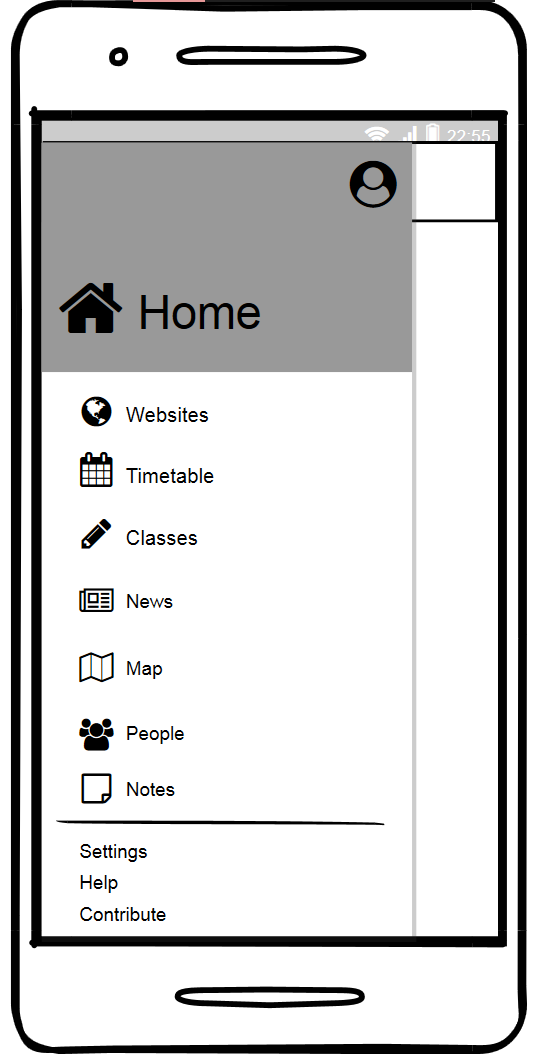
\includegraphics[width=\textwidth]{figures/app/balsamiq/drawer.png}
        \caption{Menu wireframe}
        \label{4:fig:balsamiq_menu}
    \end{minipage}
\end{figure}

We also re-drew the news page (fig. \ref{4:fig:balsamiq_news}) and added a visualization of the filtering option for this page.

\begin{figure}[!ht]
    \centering
    \begin{minipage}[t]{0.26\textwidth}
        \captionsetup{justification=centering}
        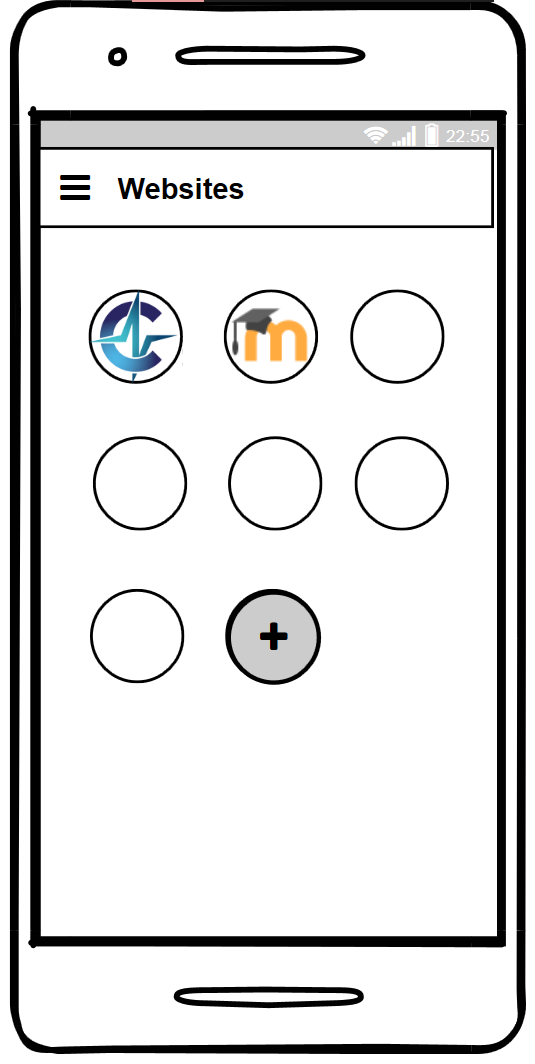
\includegraphics[width=\textwidth]{figures/app/balsamiq/websites.png}
        \caption{Websites page wireframe}
        \label{4:fig:balsamiq_websites}
    \end{minipage}
    \hfill
    \begin{minipage}[t]{0.54\textwidth}
        \captionsetup{justification=centering}
        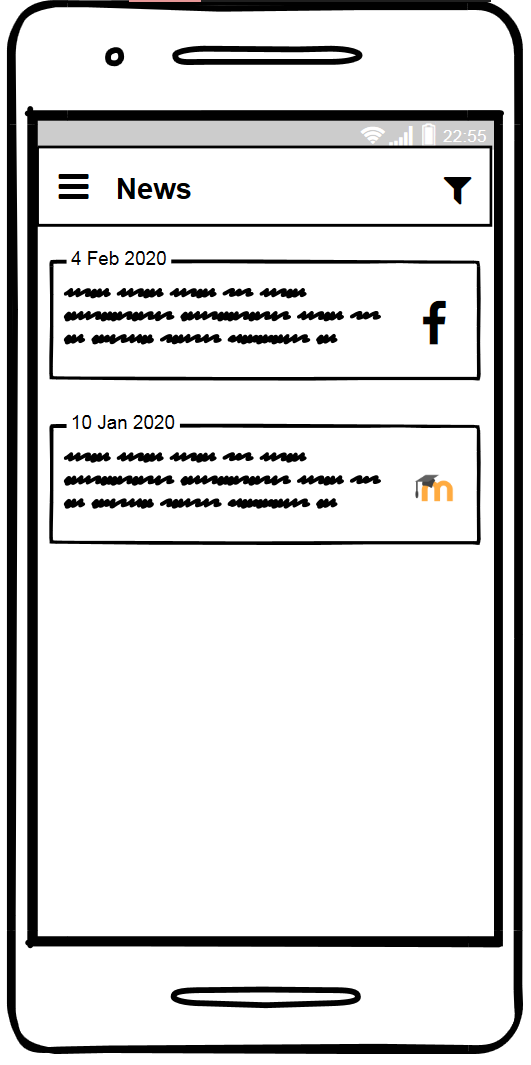
\includegraphics[width=0.485\textwidth]{figures/app/balsamiq/news.png}
        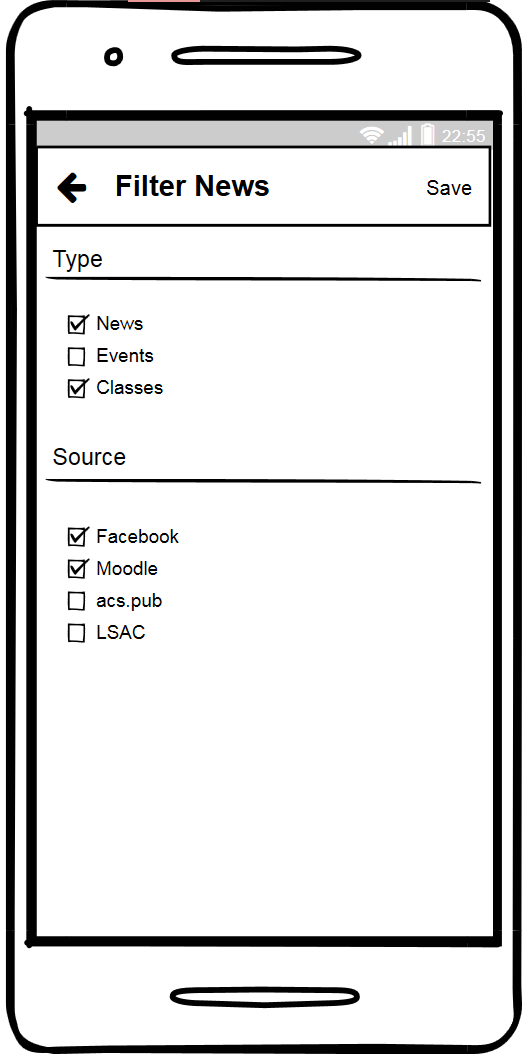
\includegraphics[width=0.49\textwidth]{figures/app/balsamiq/filter_news.png}
        \caption{News page wireframe}
        \label{4:fig:balsamiq_news}
    \end{minipage}
\end{figure}

Additionally, we added the profile page (fig. \ref{4:fig:balsamiq_profile}) requested by the feedback. It includes a potential presentation of the gamification feature suggested in section \ref{4:permissions_assigning}. This concept displays the current level of the user as well as the requirements for progressing to the next one.

We also drew the "People" page containing professor and student information (fig. \ref{4:fig:balsamiq_people}). It is pictured as a list of names and allows the user to click/tap a name to view more information about the person. It also allows filtering the list by type (student/professor).

\begin{figure}[!ht]
    \centering
    \begin{minipage}[t]{0.3\textwidth}
        \captionsetup{justification=centering}
        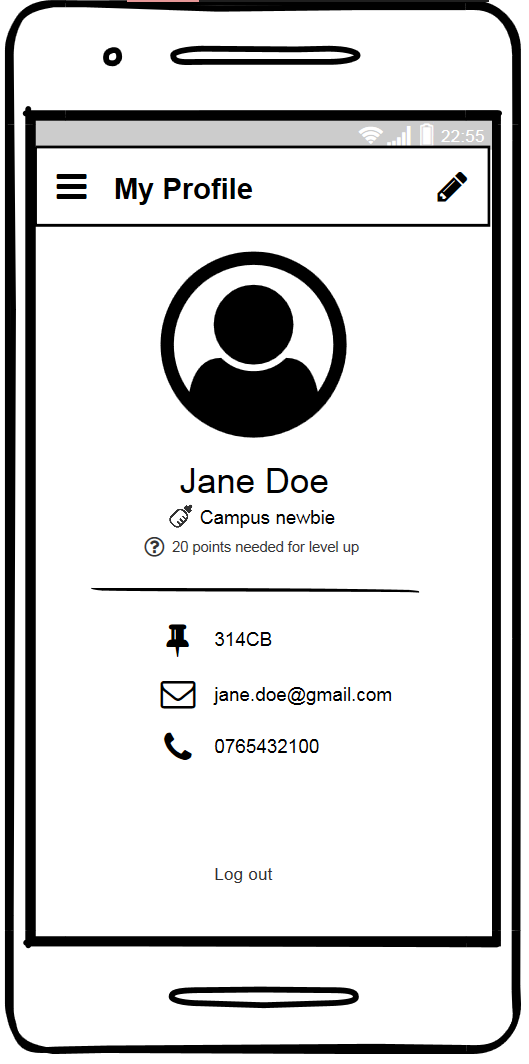
\includegraphics[width=\textwidth]{figures/app/balsamiq/profile.png}
        \caption{Profile page wireframe}
        \label{4:fig:balsamiq_profile}
    \end{minipage}
    \hfill
    \begin{minipage}[t]{0.63\textwidth}
        \captionsetup{justification=centering}
        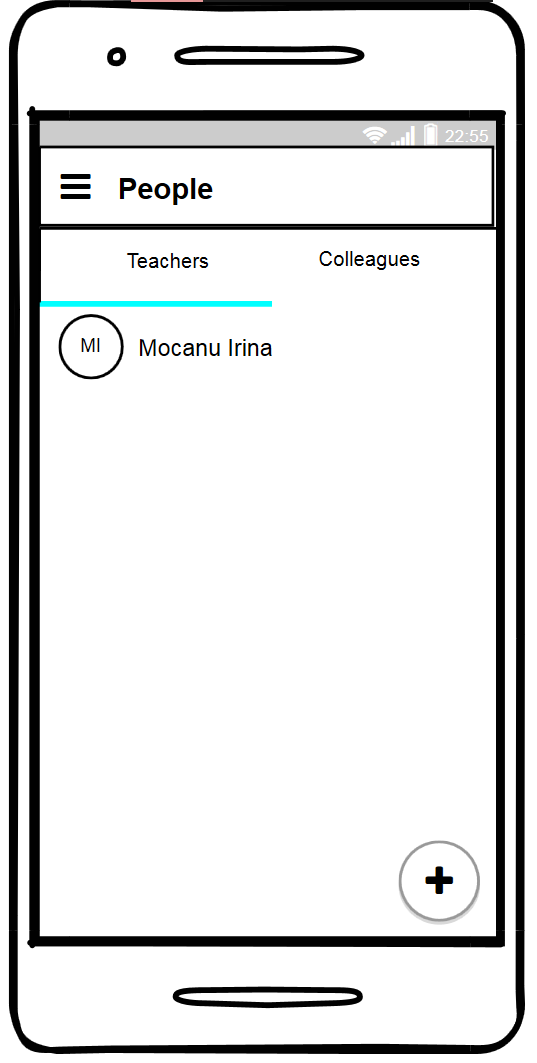
\includegraphics[width=0.485\textwidth]{figures/app/balsamiq/people.png}
        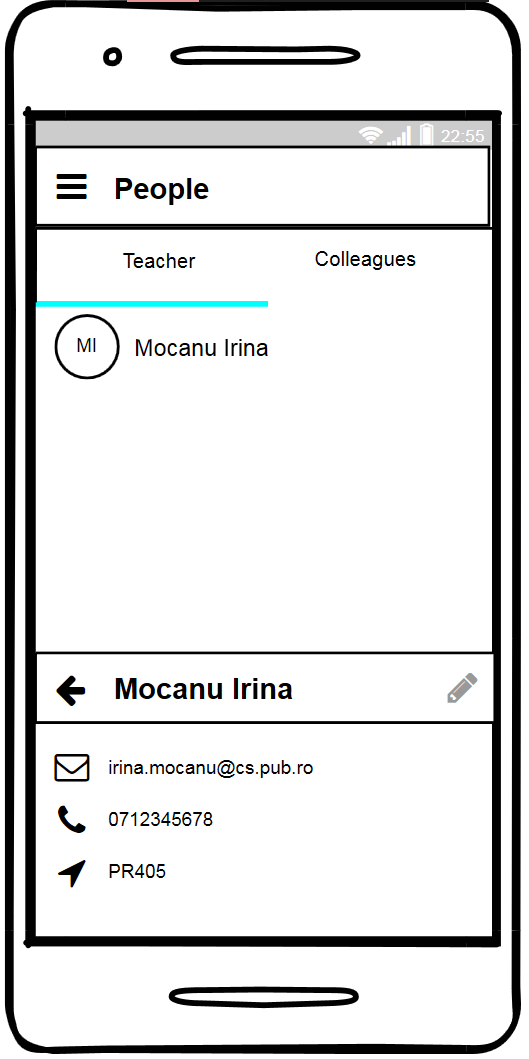
\includegraphics[width=0.48\textwidth]{figures/app/balsamiq/teacher.png}
        \caption{People page wireframe}
        \label{4:fig:balsamiq_people}
    \end{minipage}
\end{figure}

Finally, we re-designed the classes and class information pages (fig. \ref{4:fig:balsamiq_classes}) and added visualizations for the filtering mechanism as well as the entire process of adding a new event to a class (fig. \ref{4:fig:balsamiq_events}), as requested by the feedback.

Adding an event can be done by either manually inputting all data for the event (such as the name, class, and deadlines for homework) or using an event that somebody else has already created. Existing events can be voted up or down and would be automatically voted up if a user chooses to add it to their calendar in the application.

\clearpage

\begin{figure}[!ht]
    \centering
     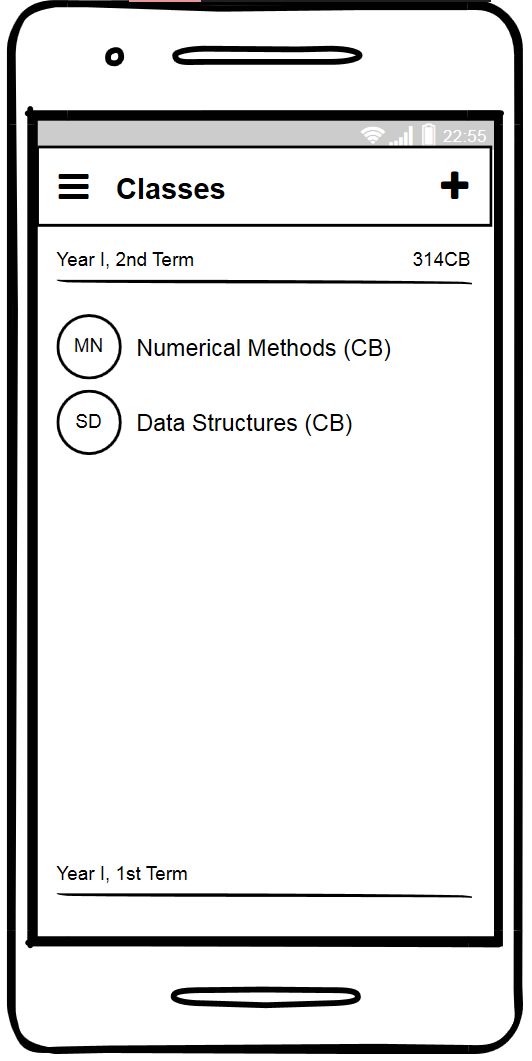
\includegraphics[width=0.32\textwidth]{figures/app/balsamiq/classes.png}
     \hfill
     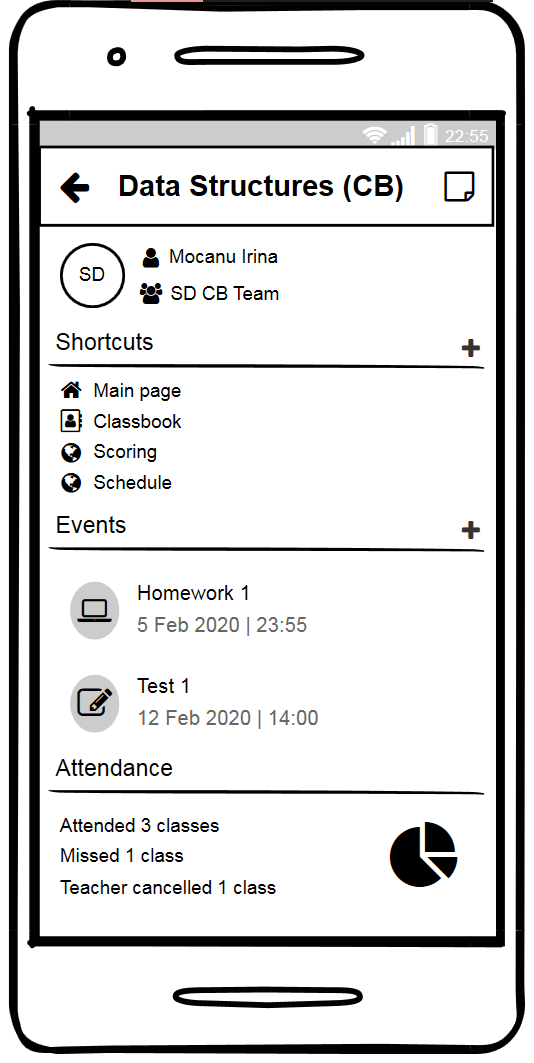
\includegraphics[width=0.32\textwidth]{figures/app/balsamiq/class_info.png}
     \hfill
     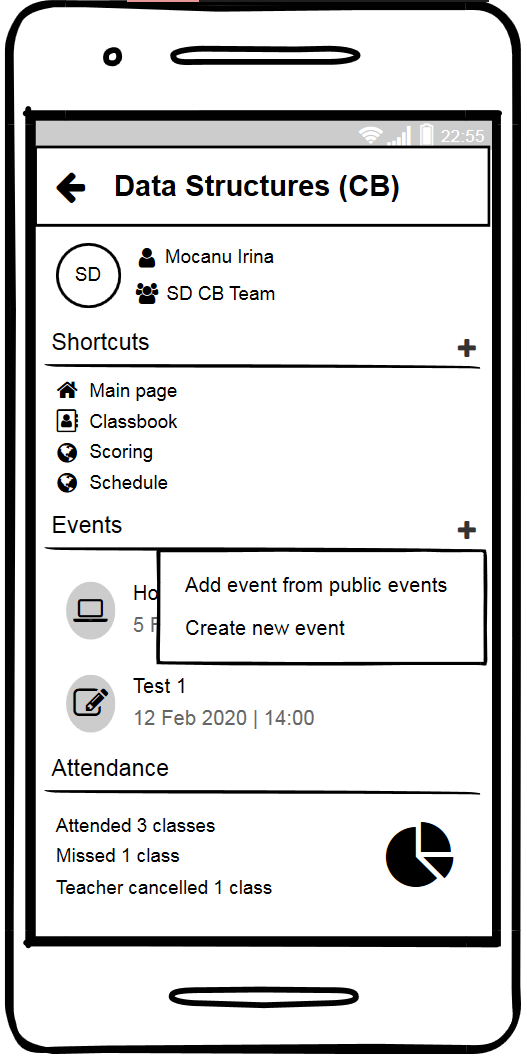
\includegraphics[width=0.32\textwidth]{figures/app/balsamiq/add_event.png}
    \caption{Classes page wireframe}
    \label{4:fig:balsamiq_classes}
\end{figure}

\begin{figure}[!ht]
    \centering
     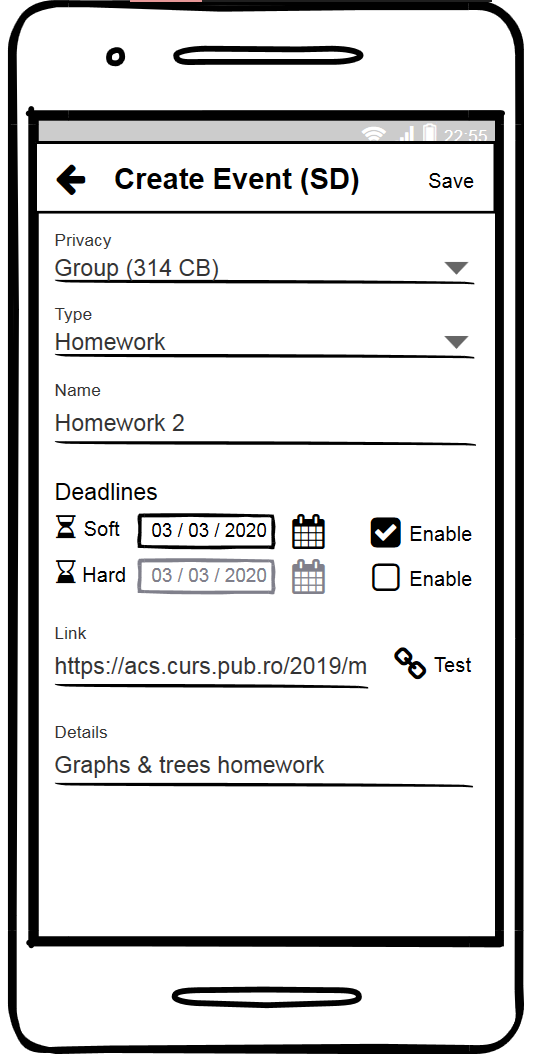
\includegraphics[width=0.32\textwidth]{figures/app/balsamiq/create_event.png}
     \hfill
     \includegraphics[width=0.32\textwidth]{figures/app/balsamiq/public_events.png}
     \hfill
     \includegraphics[width=0.32\textwidth]{figures/app/balsamiq/filter_events.png}
    \caption{Events page wireframe}
    \label{4:fig:balsamiq_events}
\end{figure}

\subsection{Feedback} \label{4:wireframe_feedback}

We asked ten students from different years to test this prototype and share their experiences. The feedback we received was very positive, with all students showing excitement about the application's features.

The students who have iOS devices pointed out that the design style is more appropriate for Android than iOS devices, which was to be expected since the main inspiration for the prototype was an Android application which uses Material Design\cite{google2020material} (\textit{School Assistant}).

\section{Final design} \label{4:final}

\subsection{Theme} \label{4:final_theme}

\begin{wrapfigure}{l}{0.15\columnwidth}
    \centering
    \includegraphics[width=0.15\columnwidth]{figures/logos/acs.png}
    \caption{\acrshort{acs} logo}
    \label{4:fig:acs_logo}
\end{wrapfigure}

For the final design, we created a dual theme (including dark \& light mode) that is inspired by the faculty logo (fig. \ref{4:fig:acs_logo}). The primary and secondary colours of the application are extracted from the logo and used for text, buttons as well as illustrations.

The font used in the application is Montserrat\footnote{https://fonts.google.com/specimen/Montserrat}.All icons are either Material Design icons\footnote{https://material.io/resources/icons/} or FontAwesome icons\footnote{https://fontawesome.com/icons/}. Illustrations are from the open-source unDraw\footnote{https://undraw.co/illustrations} gallery. All of the above are under open licenses and allow usage, modification and redistribution.

\subsection{Pages} \label{4:pages}

TODO
\chapter{Architecture} \label{chapter5}

In this chapter, we will be discussing the technologies we chose to use for this project and our implementation.

\section{Mobile technology} \label{5:technology}

\subsection{The native approach} \label{5:technology_native}

In terms of the best core technology/language to use for the mobile application itself, we initially considered a native Android solution, since the vast majority of students in the faculty (80\% according to our study, section \ref{3:target_audience}) own an Android phone. However, since our application should be available to all students, and the quality of information is dependent on the number of users in a collaborative system, a pure Android solution proved not to be the best approach.

Native mobile implementations come with various benefits, from consistent, native-compliant application design (see appendix \ref{a:native_cross}) to outstanding performance and making the best of what the device has to offer. However, having only one supported platform would mean excluding a significant number of students from the user base. On the other hand, having two separate, native implementations for each mobile OS (one written in Java/Kotlin for Android, and one written in Objective-C/Swift for iOS) would require double the amount of time and effort. Due to the complexity of the application, the native approach is regrettably out of the question.

\subsection{The cross-platform approach} \label{5:technology_cross}

Given the circumstances, we decided to look into cross-platform technologies for mobile applications. According to Sandeep Agarwal\cite{agarwal2019best}, the 5 most popular mobile app development frameworks in 2019 are React Native\footnote{https://reactnative.dev/} (by Facebook), \gls{flutter}\footnote{https://flutter.dev/} (by Google), Ionic\footnote{https://ionicframework.com/} (by Drifty), Xamarin\footnote{https://dotnet.microsoft.com/apps/xamarin} (by Microsoft) and PhoneGap\footnote{https://phonegap.com/} (by Adobe). Due to our developer not having any prior experience with JavaScript development, we decided to choose between \gls{flutter} and Xamarin. This decision is mainly influenced by the other three frameworks all being based on HTML5, CSS, and JavaScript. In terms of development language, Xamarin uses C\# and .NET, while \gls{flutter} uses Dart.

Both \gls{flutter} and Xamarin have the significant benefit of being part of a vast development ecosystem, therefore choosing the technology also implies choosing the ecosystem. \gls{flutter} is integrated within the Google ecosystem (including support for services like Google Cloud\footnote{https://cloud.google.com/} and a designated development environment: Android Studio\footnote{https://developer.android.com/studio/}). Xamarin is part of the Microsoft ecosystem (offering alternatives such as Azure Cloud Services\footnote{https://azure.microsoft.com/en-in/services/cloud-services/} and Visual Studio\footnote{https://visualstudio.microsoft.com/}).

Xamarin is a more "mature" framework with deep roots in the developer community since it was released in 2011, six years before \gls{flutter} came into the cross-platform market. However, \gls{flutter}'s community is growing rapidly, and the developers' response is overwhelmingly positive. According to the 2020 StackOverflow Developer Survey\cite{stackoverflow2020survey}, \gls{flutter} was rated the third most loved non-web framework and is the first mobile development framework in the list (with the second being React Native, and the third Xamarin).

Even though Xamarin provides support for more platforms (iOS, Android, Windows, macOS), it still requires platform-specific code for iOS and Android. For our use case (a mobile application), \gls{flutter} seems to be more appropriate since it provides better code reusability. The stable release of \gls{flutter} supports iOS and Android, while the beta and alpha channels provide web support and macOS support, respectively. A web version of a \gls{flutter} application can be run on any web-enabled device (including Windows and Linux devices, for which native support is still under development). Therefore we believe that \gls{flutter} appropriately meets the need for our application to be readily available for any student.

Upon careful consideration of the leading cross-platform technologies available for developing mobile applications, we have concluded that \textbf{\gls{flutter}} is the best technology for our application.

\section{Database} \label{5:database}

Being part of the Google ecosystem, \gls{flutter} offers seamless integration with the Google Cloud Platform and other Google services such as \gls{firebase}\footnote{https://firebase.google.com/}. For mobile applications, \gls{firebase} offers features such as analytics, database, and authentication, therefore we have decided to take advantage of it for all of our cloud-based needs.

\subsection{Firestore} \label{5:firestore}
Cloud Firestore\footnote{https://firebase.google.com/docs/firestore/} is a \gls{nosql} database that organises its data in \textit{collections} and \textit{documents}.

\subsubsection{Data model} \label{5:firestore_data_model}
\textbf{Collections} are simply a list of documents, where each document has an ID within the collection.

\textbf{Documents} are similar to a \gls{json} file, in that they contain different fields which have three important components: a \textit{name} - what we use to refer to the field, similar to a dictionary key -, a \textit{type} (which can be one of \mintinline{text}{string}, \mintinline{text}{number}, \mintinline{text}{boolean}, \mintinline{text}{map}, \mintinline{text}{array}, \mintinline{text}{null}, \mintinline{text}{timestamp}, \mintinline{text}{geopoint}, \mintinline{text}{reference}), and the actual \textit{value}, the data contained in the field.
In addition to fields, documents can contain collections, which in turn contain other documents, thus allowing us to create a hierarchical structure within the database.

\subsubsection{Security} \label{5:firestore_security}
Firestore allows for defining specific security rules for each collection. Rules can be applied for each different type of transaction - \mintinline{text}{read}s (where single-document reads - \mintinline{text}{get} - and queries - \mintinline{text}{list} - can have different rules) and \mintinline{text}{write}s (where \mintinline{text}{create}, \mintinline{text}{delete} and \mintinline{text}{update} can be treated separately).

\subsection{Authentication} \label{5:authentication}
\gls{firebase} provides an entire suite of back-end services and \acrshort{sdk}s for authenticating users within an application, through FirebaseAuth\footnote{https://firebase.google.com/docs/auth}.

For our application, we use the following features:
\begin{itemize}
    \setlength{\topsep}{0.5pt}
    \setlength{\itemsep}{0.5pt}
    \setlength{\parsep}{0.5pt}
    \item account creation
    \item login
    \item password reset via e-mail
    \item account verification via e-mail
    \item account deletion
\end{itemize}

The class structure can be seen in appendix \ref{a:uml}, figure \ref{a:fig:uml_authentication}. The \mintinline{dart}{AuthProvider} class is responsible for communicating with FirebaseAuth.

This service automatically handles the authentication tokens and enforces security rules, which is particularly useful for an open-source application which users can fiddle with, such as ours. For example, multiple failed authentication attempts lead to a temporary timeout, and a user cannot delete their account unless they have logged in very recently (or refreshed their authentication token).

Firestore security rules (see subsection \ref{5:firestore_security}) can be enforced based on the user's \acrshort{uid}. This method means that, even though users can access the database connection string through the public repository, they can only do a limited set of actions on the database, depending on whether they are authenticated and their rights.

\subsection{Project database structure} \label{5:database_project}
We opted for a database architecture where all documents within a collection can contain a subset of fields from a given list, similar to a relational database table. Some fields are required to be present (similar to \mintinline{sql}{NOT NULL} columns in a \textit{SQL} database), while others might not be present (similar to a column with the \mintinline{sql}{NULL} property). This structure makes it easier to migrate to a relational database in the future, should the need arise.

The project database contains the following collections:

~

\faDatabase \hspace{0.1cm} \textbf{\mintinline{text}{users}}

This collection stores per-user data. The document key is the user's \mintinline{text}{uid} (from FirebaseAuth, see subsection \ref{5:authentication}).

All the documents in the collection share the structure described in table \ref{5:tab:users}.

\begin{table}[th]\small\linespread{1}
\caption{\textbf{users} collection structure}
\label{5:tab:users}
\begin{tabular}{| l | l | c | p{4.7cm} |}
\hline
\textbf{Field} & \textbf{Type} & \textbf{Required?} & \textbf{Additional info} \\
\hline
group & \mintinline{text}{string} & \Checkedbox & e.g. "314CB" 
\\
\hline
name & \mintinline{text}{map<string, string>} & \Checkedbox & keys are "first" and "last"
\\
\hline
permissionLevel & \mintinline{text}{number} & \CrossedBox & a numeric value that defines what the user is allowed to do; if missing, it is treated as being equal to zero
\\
\hline
\end{tabular}
\end{table}

A user can define their private events and websites, that only they can access. These will reside in the \textbf{events} and \textbf{websites} sub-collections, respectively, which have a similar structure as the root-level collections with the same names, described below in this section.

We define special \textit{\textbf{rules}} (see subsection \ref{5:firestore_security}) for this collection and its subcollections. Anyone can create a new user (a new document in this collection) if the \textit{permissionLevel} of the created user is \mintinline{text}{0}, \mintinline{text}{null} or not set at all. Authenticated users can only \mintinline{text}{read}, \mintinline{text}{delete} and \mintinline{text}{update} their own document (including its subcollections) and no one else's. However, they cannot modify the \textit{permissionLevel} field.

\clearpage

\faDatabase \hspace{0.1cm} \textbf{\mintinline{text}{websites}}

This collection stores useful websites, shown in the app under the \textbf{Portal} page. Which students they are relevant for depends on the \textit{degree} and \textit{relevance} fields (for more information, see the \textbf{filters} collection described below in this section).

The documents in this collection share the structure pictured in table \ref{5:tab:websites}.

\begin{table}[th]\small\linespread{1}
\caption{\textbf{websites} collection structure}
\label{5:tab:websites}
\begin{tabular}{| l | p{2.6cm} | c | p{7.1cm} |}
\hline
\textbf{Field} & \textbf{Type} & \textbf{Required?} & \textbf{Additional info} \\
\hline
category & \mintinline{text}{string} & \Checkedbox & one of: “learning”, “association”, “administrative”, “resource”, “other”
\\
\hline
degree & \mintinline{text}{string} &    \HollowBox & “BSc” or “MSc”, must be specified if \textit{relevance} is not \mintinline{text}{null}
\\
\hline
editedBy & \mintinline{text}{array<string>} & \CrossedBox & list of user IDs
\\
\hline
icon & \mintinline{text}{string} & \CrossedBox & path in Firebase Storage; if missing, it defaults to "icons/websites/globe.png"
\\
\hline
label & \mintinline{text}{string} & \Checkedbox & unless specified, the app sets this to be the link without the protocol
\\
\hline
link & \mintinline{text}{string} & \Checkedbox & it needs to include the protocol (\textit{http://}, \textit{https://} etc.)
\\
\hline
relevance & \mintinline{text}{null} /

\mintinline{text}{list<string>}& \Checkedbox & \mintinline{text}{null}\footnotemark if relevant for everyone, otherwise a string of filter node names
\\
\hline
\end{tabular}
\end{table}

\footnotetext{In Firestore, \mintinline{text}{null} is a data type; a field that is \mintinline{text}{null} is different from a field that is not present in a document.}

This collection also has a special set of \textbf{rules}\textit{} (see subsection \ref{5:firestore_security}), based on the permission levels described in section \ref{4:permissions_levels}. Since websites in this collection are public information (anyone can \mintinline{text}{read}), altering and adding data here is a privilege and needs to be monitored, therefore anyone who wants to modify this data needs to be authenticated in the first place. Users can \mintinline{text}{create} a new public website only if their \textit{permissionLevel} is equal to or greater than two  and they sign the data by putting their \textit{uid} in the \textit{addedBy} field. Users can \mintinline{text}{update} a website if they do not modify the \textit{addedBy} field and they sign the modification by adding their \textit{uid} at the end of the \textit{editedBy} list. Users can only delete a website if they are the ones who created it (their \textit{uid} is equal to the addedBy field) or if their \textit{permissionLevel} is equal to or greater than three.

\clearpage

\faDatabase \hspace{0.1cm} \textbf{\mintinline{text}{filters}}

This collection stores \mintinline{dart}{Filter} objects. These are essentially trees with named nodes and levels. In the case of the relevance filter, they are meant to represent the way the University organizes students:

\begin{minted}{text}
                              All
                _______________|______________
              /                                \
            BSc                               MSc // Degree
     ________|________                 ________|__ ...
   /                  \              /     |
  IS                 CTI            IA   SPRC ... // Specialization
..|..           ______|______       ⋮      ⋮
              /    |     |   \
           CTI-1 CTI-2 CTI-3 CTI-4                // Year
              ⋮    ⋮   __|... ⋮
                    /   |
                 3-CA 3-CB ...                    // Series
                 __|...
               /   |
           331CA 332CA ...                        // Group
\end{minted}

The tree-based structure is defined using \mintinline{text}{map}s, as pictured in table \ref{5:tab:filters}.

\begin{table}[th]\small\linespread{1}
\caption{\textbf{filters} collection structure}
\label{5:tab:filters}
\begin{tabular}{| l | p{2.6cm} | c | p{7.1cm} |}
\hline
\textbf{Field} & \textbf{Type} & \textbf{Required?} & \textbf{Additional info} \\
\hline
levelNames & \mintinline{text}{array<}

\mintinline{text}{ map<string,}

\mintinline{text}{  string>>} & \Checkedbox & localized names for each tree level (e.g. "Year"); the map keys are the locale strings ("en", "ro")
\\
\hline
root & \mintinline{text}{map<string,}

\mintinline{text}{ map<string,}

\mintinline{text}{  map<...>>>} & \Checkedbox & nested map representing the tree structure, where the key is the name of the node and the value is a map of its children
\\
\hline
\end{tabular}
\end{table}

The filter structure is public information and should never (or very rarely) need to be modified, therefore for this collection, anyone can \mintinline{text}{read}, but no one can \mintinline{text}{write}.

~

\faDatabase \hspace{0.1cm} \textbf{\mintinline{text}{classes}}

This collection contains information about the classes taught in the faculty, its structure being pictured in table \ref{5:tab:classes}. Classes are taught in a specific year during a specific semester. While some are taught by the same professor (and have the same rules) for a whole generation, others are split on student series. In order to represent this, a \textbf{class} document can contain a \textbf{subclasses} collection which splits the information that can differ by series (fig. \ref{5:tab:classes/subclasses}). 

\begin{table}[th]\small\linespread{1}
\caption{\textbf{classes} collection structure}
\label{5:tab:classes}
\begin{tabular}{| l | p{2.6cm} | c | p{7.3cm} |}
\hline
\textbf{Field} & \textbf{Type} & \textbf{Required?} & \textbf{Additional info} \\
\hline
acronym & \mintinline{text}{string} & \Checkedbox & unique class acronym according to the \gls{moodle} page
\\
\hline
class & \mintinline{text}{string} & \Checkedbox & official class name
\\
\hline
degree & \mintinline{text}{string} & \Checkedbox & degree where the class is taught
\\
\hline
domain & \mintinline{text}{string} & \Checkedbox & domain where the class is taught
\\
\hline
semester & \mintinline{text}{string} & \Checkedbox & semester in which the class is taught
\\
\hline
year & \mintinline{text}{string} & \Checkedbox & academic year in which the class is taught
\\
\hline
lecturer & \mintinline{text}{string} & \CrossedBox & lecturer that teaches the class
\\
\hline
shortcuts & \mintinline{text}{array<}

\mintinline{text}{ map<string,}

\mintinline{text}{  string>>} & \CrossedBox & links to relevant resources, similar to websites on the portal page (keys are "name", "link", "addedBy" and "type" - one of "main", "classbook", "resource", "other")
\\
\hline
\end{tabular}
\end{table}

\begin{table}[th]\small\linespread{1}
\caption{\textbf{classes/subclasses} subcollection structure}
\label{5:tab:classes/subclasses}
\begin{tabular}{| l | p{2.6cm} | c | p{7.3cm} |}
\hline
\textbf{Field} & \textbf{Type} & \textbf{Required?} & \textbf{Additional info} \\
\hline
series & \mintinline{text}{string} & \Checkedbox & series where the class is taught
\\
\hline
lecturer & \mintinline{text}{string} & \CrossedBox & lecturer that teaches the class
\\
\hline
shortcuts & \mintinline{text}{array<}

\mintinline{text}{ map<string,}

\mintinline{text}{  string>>} & \CrossedBox & links to relevant resources, similar to websites on the portal page (keys are "name", "link" and "type" - one of "main", "classbook", "resource", "other")
\\
\hline
\end{tabular}
\end{table}

Most of this information almost never changes from year to year, therefore students with at least \textit{permissionLevel} 3 (see section \ref{4:permissions_levels}) can only add or remove resource links (namely, the \textit{shortcuts} field).

\clearpage

\faDatabase \hspace{0.1cm} \textbf{\mintinline{text}{events}}

This collection contains timetable events. Depending on the event type, it will have a different set of relevant fields in its document. For example, recurring events such as laboratories and lectures will be defined by a \textit{start} and \textit{end} day and a recurrence rule (\textit{rrule}) and have an associated \textit{location}. Homeworks will not have a location, but rather have a \textit{soft} and \textit{hard} deadline as well as a \textit{name} and a \textit{link}. Most events will have a \textit{class} associated with them (see the \textbf{classes} collection described above).

\begin{table}[th]\small\linespread{1}
\caption{\textbf{events} collection structure}
\label{5:tab:events}
\begin{tabular}{| l | p{2cm} | c | p{7.5cm} |}
\hline
\textbf{Field} & \textbf{Type} & \textbf{Required?} & \textbf{Additional info} \\
\hline
type & \mintinline{text}{string} & \Checkedbox & one of "lab", "seminar", "lecture", "sports", "exam", "homework", "project", "test", "practical", "research"
\\
\hline
class & \mintinline{text}{string} & \CrossedBox & document ID of a class in the \textbf{classes} collection
\\
\hline
start & \mintinline{text}{timestamp} & \CrossedBox & a start date, where applicable (e.g. beginning of the semester)
\\
\hline
end & \mintinline{text}{timestamp} & \CrossedBox & an end date, where applicable (e.g. end of the semester)
\\
\hline
rrule & \mintinline{text}{string} & \CrossedBox & recurrence rule (e.g. "weekly", "bi-weekly")
\\
\hline
location & \mintinline{text}{string} & \CrossedBox & location where the event takes place, if applicable
\\
\hline
description & \mintinline{text}{string} & \CrossedBox & event description, if relevant
\\
\hline
name & \mintinline{text}{string} & \CrossedBox & event name, if applicable (labs/lectures don't have a name)
\\
\hline
soft & \mintinline{text}{timestamp} & \CrossedBox & soft deadline (for homework)
\\
\hline
hard & \mintinline{text}{timestamp} & \CrossedBox & hard deadline (for homework)
\\
\hline
\end{tabular}
\end{table}

This collection has the same permissions as the \textbf{websites} collection described above.

\clearpage

\faDatabase \hspace{0.1cm} \textbf{\mintinline{text}{people}}

Public information about people (particularly faculty members) is available in this collection. It is currently immutable and can only be read by any user since it is extracted from the faculty information website\footnote{https://cs.pub.ro/index.php/?option=com\_comprofiler\&task=userslist\&listid=2}, but in the future, it can be modified depending on the user's permissions. The structure of this information is described in table \ref{5:tab:people}.

\begin{table}[th]\small\linespread{1}
\caption{\textbf{people} collection structure}
\label{5:tab:people}
\begin{tabular}{| l | p{1.3cm} | c | p{8.7cm} |}
\hline
\textbf{Field} & \textbf{Type} & \textbf{Required?} & \textbf{Additional info} \\
\hline
name & \mintinline{text}{string} & \Checkedbox & the person's full name
\\
\hline
email & \mintinline{text}{string} & \CrossedBox & the person's e-mail address
\\
\hline
office & \mintinline{text}{string} & \CrossedBox & the person's office, if applicable
\\
\hline
photo & \mintinline{text}{string} & \CrossedBox & a link to the person's photo
\\
\hline
position & \mintinline{text}{string} & \CrossedBox & the person's position (e.g. "Student", "Lecturer" etc.)
\\
\hline
\end{tabular}
\end{table}

\section{System design \& implementation} \label{5:implementation}

The entire system is fairly complex (figure \ref{a:fig:uml} in appendix \ref{a:uml} shows a simplified UML diagram that does not include the localization class). We will not describe it in detail, but rather focus on describing the top-level components and the main design pattern used to implement them.

\subsection{Primary components}
The main components of the architecture are linked to its features:
\begin{itemize}
    \setlength{\topsep}{0.5pt}
    \setlength{\itemsep}{0.5pt}
    \setlength{\parsep}{0.5pt}
    \item the \textbf{authentication} component uses FirebaseAuth (see subsection \ref{5:authentication}) to allow the student to make various account management actions
    \item the \textbf{page} components deal with each of the application's pages (see section \ref{4:pages}) and handle their specific data
\end{itemize}

\subsection{State management} \label{5:state_management}
\mintinline{dart}{Provider} is a dependency injection framework which can be used to manage state in a \gls{flutter} application.

To understand how \mintinline{dart}{Provider} works, we first need to understand the structure of a \gls{flutter} application. \gls{flutter} \acrshort{ui} revolves around widgets, which are components controlling some part of the interface. Widgets are organized in a tree structure, with parent widgets controlling the behavior of their children. Widgets are partly similar to HTML tags - for example, a widget containing a bit of text can be centered by wrapping it inside a \mintinline{dart}{Center} widget (see table \ref{5:tab:flutter_html}).

\begin{table}[th]\small\linespread{1}
\caption{Tree-based structure of HTML and \gls{flutter}}
\label{5:tab:flutter_html}
\begin{tabular}{| m{0.45\textwidth} | m{0.45\textwidth} |}
\hline
\textbf{HTML} & \textbf{\gls{flutter}} \\
\hline
\begin{minted}
[
framesep=0mm
]
{html}
<center>
    <h1>Hello, world!</h1>
</center>
\end{minted}
&
\begin{minted}{dart}
Center(
    child: Text(
        "Hello, world!",
        textTheme.headline1,
    );
);
\end{minted}
\\
\hline
\end{tabular}
\end{table}

\mintinline{dart}{Provider}s offer an easy way to encapsulate state and share it with a branch of the widget tree. It achieves that by being defined as the parent of that branch. Alternatively, if the whole application requires access to a specific state (as is the case of authentication in our application), the \mintinline{dart}{Provider} needs to be defined as the parent of the entire widget tree:

\begin{minted}{dart}
runApp(ChangeNotifierProvider<AuthProvider>(
      create: (_) => AuthProvider(), child: MyApp()));
\end{minted}

\subsection{Separation of concerns} \label{5:separation}

For each component, we use a variant of the \gls{bloc} (Business Logic Component) design pattern which utilizes \mintinline{dart}{Provider} (described in the previous subsection, \ref{5:state_management}) in order to avoid boilerplate code.

\begin{wrapfigure}{r}{.25\columnwidth}
    \centering
    \includegraphics[width=.25\columnwidth]{figures/bloc.png}
    \caption{Standard \gls{bloc} architecture}
    \label{5:fig:bloc}
\end{wrapfigure}

Figure \ref{5:fig:bloc} shows the classic \gls{bloc} structure. Based on this pattern, each page in our application is made up of three main components:
\begin{itemize}
    \setlength{\topsep}{0.5pt}
    \setlength{\itemsep}{0.5pt}
    \setlength{\parsep}{0.5pt}
    \item the \textbf{\acrshort{ui}/\gls{flutter} layer}, also called the \textbf{view}, which acts as a middleman between the user and the \gls{bloc} layer
    \item the \textbf{\gls{bloc} layer}, which we also refer to as the \textbf{\mintinline{dart}{Provider}} or \textbf{service}, contains the actual business logic and communicates with the database
    \item the \textbf{data layer} or the data \textbf{model} contains simple data classes which represent the data that is to be displayed in the \acrshort{ui}, and is provided by the \gls{bloc}
\end{itemize}

For example, the portal page has three main components, which can be observed in appendix \ref{a:uml}, figure \ref{a:fig:uml_portal}. The \textbf{view} manages the \acrshort{ui} and includes both the page listing the websites as well as the form page allowing users to add/modify a website. The \textbf{model} is the \mintinline{dart}{Website} data class and contains all of the relevant fields for a website (e.g., name, link, localized information, path to the icon). The \textbf{service} is a \mintinline{dart}{ChangeNotifierProvider} and is responsible for fetching the data from Firestore and converting it to a list of \mintinline{dart}{Website}s. The service also checks the validity of new data and sends it to the server to be updated.

\subsection{Localization} \label{5:localization}
Thanks to our user study, we know that Romanian and English localization is essential for a large portion of our potential user base (see section \ref{3:language} for the relevant survey results). Therefore, we implemented localization using \gls{flutter}-compatible tools.

The application's localized strings are defined in .ARB (App Resource Bundle)\footnote{https://github.com/google/app-resource-bundle} files, a simple localization resource format based on \gls{json} and introduced by Google. The \textit{Fluter Intl}\footnote{https://plugins.jetbrains.com/plugin/13666-flutter-intl} Android Studio plugin automatically generates \textit{Dart Intl}\footnote{https://pub.dev/packages/intl} boilerplate code which binds the \gls{flutter} application to the translations in the .ARB files.

\section{\acrshort{ci} \& \acrshort{cd}} \label{5:cicd}

\subsection{Testing} \label{5:cicd_testing}

A test-driven approach is necessary for any medium to large project with multiple contributors, to ensure that new changes work as intended and do not break existing features. It has been shown\cite{hilton2009quantitatively} to improve code quality and maintainability significantly.

We decided to use the \mintinline{dart}{flutter_test} library\footnote{https://api.flutter.dev/flutter/flutter\_test/flutter\_test-library.html} to test our application. The \gls{bloc} architecture (described in section \ref{5:separation}) makes it easy to test each individual component. We focused on testing the data and UI layers, since the service layer mostly calls methods from the \mintinline{dart}{flutterfire} plugin\footnote{https://github.com/FirebaseExtended/flutterfire} which connects to Firestore. The Firestore plugin is already heavily tested by its developers and would be complicated to mock. As a result, more than 70\% (fig. \ref{5:fig:codecov}), the application code is being tested through over 200 unit and integration tests. We aim to keep this number above the 60\% threshold.

\begin{figure}[!ht]
    \centering
     \includegraphics[width=0.95\textwidth]{figures/charts/codecov.png}
     \caption{Application code coverage according to \textit{codecov}}
    \label{5:fig:codecov}
\end{figure}

\subsection{Deployment} \label{5:cicd_deployment}
The application is currently being hosted on the web using two free Firebase domains\footnote{https://acs-upb-mobile.web.app/ and https://acs-upb-mobile.firebaseapp.com/}. Deployment is done through the \mintinline{shell}{firebase deploy} command of the Firebase \acrshort{cli}\footnote{https://firebase.google.com/docs/cli}.

In the future, the mobile application can be published directly onto the App Store and Google Play (see subsection \ref{6:future_publish}) for easy access.

\subsection{GitHub Actions} \label{5:cicd_actions}

The code of the application is public in a GitHub repository\footnote{https://github.com/acs-upb-mobile/acs-upb-mobile/}, which makes it easy for students to contribute by creating an issue or submitting a \acrshort{pr}. GitHub allows setting up an automated testing and deployment pipeline using GitHub Actions\footnote{https://github.com/features/actions/}, which is what we chose to use for our application.

For \acrlong{ci} (\acrshort{ci}), we created a workflow\footnote{https://github.com/acs-upb-mobile/acs-upb-mobile/blob/master/.github/workflows/test.yml} which runs on every push to the repository. It runs all tests (see subsection \ref{5:cicd_testing}) on an Ubuntu virtual machine and sends coverage information to \textit{codecov}\footnote{https://codecov.io/gh/acs-upb-mobile/acs-upb-mobile}. 

For \acrlong{cd} (\acrshort{cd}), we defined a deployment workflow\footnote{https://github.com/acs-upb-mobile/acs-upb-mobile/blob/master/.github/workflows/deploy.yml} which is triggered on the creation of a new tag. It runs all tests and, if they succeed, builds and publishes the web version (see subsection \ref{5:cicd_deployment}) onto the Firebase servers and creates a new release on GitHub containing the built APK for Android devices.

% Include abbreviations
\clearpage
\addcontentsline{toc}{chapter}{Abbreviations}
\printglossary[title=Abbreviations,type=\acronymtype]
\newpage

% Include glossary
\clearpage
\addcontentsline{toc}{chapter}{Glossary}
\printglossary

% Include bibliography
\clearpage
\addcontentsline{toc}{chapter}{Bibliography}
\bibliographystyle{IEEEtran}
\bibliography{bibliography}

% Include appendix
\begin{appendices}
\addtocontents{toc}{\protect\setcounter{tocdepth}{1}}
\makeatletter
\addtocontents{toc}{%
  \begingroup
  \let\protect\l@chapter\protect\l@section
  \let\protect\l@section\protect\l@subsection
}
\makeatother

\chapter{Native versus cross-platform appearance} \label{a:native_cross}

    \begin{figure}[ht]
        \centering
             \includegraphics[width=0.95\textwidth]{figures/reddit/reddit_web.png}
        \caption{Official Reddit website}
        \label{a:fig:reddit_web}
    \end{figure}
  
    \begin{figure}[ht]
        \centering
             \includegraphics[width=\textwidth]{figures/reddit/reddit_android.png}
        \caption{Official Android Reddit application}
        \label{a:fig:reddit_android}
    \end{figure}
    
    \begin{figure}[ht]
        \centering
             \includegraphics[width=\textwidth]{figures/reddit/reddit_boost.png}
        \caption{Boost for Reddit, an unofficial Android application}
        \label{a:fig:reddit_boost}
    \end{figure}
    
    \begin{figure}[ht]
        \centering
             \includegraphics[width=\textwidth]{figures/reddit/reddit_ios.png}
        \caption{Official iOS Reddit application}
        \label{a:fig:reddit_ios}
    \end{figure}
    
    \begin{figure}[ht]
        \centering
             \includegraphics[width=\textwidth]{figures/reddit/reddit_apollo.png}
        \caption{Apollo for Reddit, an unofficial iOS application}
        \label{a:fig:reddit_apollo}
    \end{figure}

\begin{landscape}
\chapter{UML diagrams} \label{a:uml}
    \begin{figure}[ht]
        \centering
             \includegraphics[width=\linewidth]{figures/uml/system.pdf}
        \caption{A simplified UML diagram of the entire system}
        \label{a:fig:uml}
    \end{figure}
    
    \begin{figure}[ht]
        \centering
             \includegraphics[width=\linewidth]{figures/uml/portal.pdf}
        \caption{Diagram of the portal page}
        \label{a:fig:uml_portal}
    \end{figure}
    
    \begin{figure}[ht]
        \centering
             \includegraphics[width=\linewidth]{figures/uml/authentication.pdf}
        \caption{Diagram of the authentication system}
        \label{a:fig:uml_authentication}
    \end{figure}
\end{landscape}
    
\addtocontents{toc}{\endgroup}
\end{appendices}

\end{document}